% pii — Architecture and Development Manual
% Template: kaobook · compiled through lnx's texlive container
\documentclass[
	fontsize=10pt,
	twoside=false,
	secnumdepth=2,
	open=any,
]{kaobook}

\usepackage[english]{babel}
\usepackage[style=english]{csquotes}
\usepackage{amsmath, amssymb}
\usepackage{booktabs}
\usepackage{longtable}
\usepackage{array}
\usepackage{listings}
\usepackage{xcolor}
\usepackage{hyperref}

% TikZ: every concept in these manuals is drawn, not only described.
\usepackage{tikz}
\usetikzlibrary{arrows.meta, positioning, calc, shapes.geometric, shapes.misc,
                fit, backgrounds, patterns, decorations.pathreplacing}
\usepackage{pgfplots}
\pgfplotsset{compat=1.18}

% One visual vocabulary for both manuals, so a box means the same thing in every figure.
\tikzset{
  box/.style={draw, rounded corners=2pt, fill=blue!4, align=center,
              inner sep=4pt, font=\footnotesize, minimum height=1.0cm},
  store/.style={draw, cylinder, shape border rotate=90, aspect=0.25, fill=orange!8,
                align=center, inner sep=3pt, font=\footnotesize, minimum height=1.1cm},
  model/.style={draw, rounded corners=8pt, fill=purple!8, align=center,
                inner sep=4pt, font=\footnotesize, minimum height=1.0cm},
  verdict/.style={draw, diamond, aspect=1.6, fill=green!8, align=center,
                  inner sep=1pt, font=\scriptsize},
  port/.style={font=\scriptsize\itshape, inner sep=1pt, fill=white},
  flow/.style={-{Latex[length=2mm]}, thick},
  soft/.style={-{Latex[length=2mm]}, thick, dashed, gray!70},
  back/.style={-{Latex[length=2mm]}, thick, red!60!black, dashed},
  group/.style={draw, dashed, rounded corners=4pt, inner sep=8pt, gray!60},
}


\definecolor{codebg}{RGB}{247,247,249}
\lstset{
	basicstyle=\ttfamily\footnotesize,
	backgroundcolor=\color{codebg},
	frame=single,
	framesep=3pt,
	breaklines=true,
	columns=fullflexible,
	keepspaces=true,
	showstringspaces=false,
	postbreak=\mbox{\textcolor{gray}{$\hookrightarrow$}\space},
}

\titlehead{pii \textperiodcentered{} personal information index}
\title{Architecture and Development Manual}
\author{Marcelo Correa}
\date{Version 0.2.0 \textperiodcentered{} 4 November 2026}
\publishers{The internals: engine, composition, stores, gates}

\begin{document}

\frontmatter
\maketitle

\uppertitleback{\titlehead}
\lowertitleback{
	\textbf{About this manual} \\
	This is the developer's book. It explains how pii is built and why each piece is
	shaped the way it is, including the parts that were rebuilt after they failed in
	production. The companion volume, \textit{pii --- User and Administration Manual},
	covers installation and daily use.

	\medskip
	\textbf{How it was written} \\
	Every mechanism here was read from the code and then exercised: the exit rule in
	composition was found by a graph whose refusal vanished; the retention guard by a
	fixture that was deleted; the gate's environment leak by a control that passed in
	one place and failed in another.

	\medskip
	\textbf{Version} \\
	Measured against pii 0.2.0 and the nineteen rows that landed with it.

	\medskip
	\textbf{Colophon} \\
	Typeset with \LaTeX{} using the \href{https://www.latex-templates.com/template/kaobook}{kaobook}
	template, compiled through the shared texlive container on \texttt{lnx}.
}

\tableofcontents

\mainmatter
\chapter{Design goals}

\label{ch:design-goals}

This chapter answers a single question: what is pii \emph{for}, and which constraints follow from
that purpose whether or not anyone likes them. Every later chapter describes a mechanism; this one
describes the pressure that shaped it. The purpose is narrow. pii exists so that a claim about work
a model did --- \enquote{the spec is implemented}, \enquote{the tests pass}, \enquote{the document
is current} --- can be checked by someone who was not present, from records the system kept while
it worked. Everything else in the workspace is downstream of that.

The book is deliberately organised around failure. Each of the five chapters that follow names the
mechanism \emph{and} the defect that made the mechanism necessary, because in this repository the
two are not separable: the exit rule in composition exists because a refusal silently vanished, the
health record exists because a status was being recomputed from 41{,}150 events on every call, and
the queue's lease exists because one dead claim wedged an entire lane. A design goal that has never
cost anybody anything is a slogan. The ones below have all been paid for.

\section{The four goals}

\begin{enumerate}
	\item \textbf{Evidence over narration.} A run leaves a journal of transitions; the stores keep
	counters and headers. A statement that cannot be reconstructed from those records is treated as
	unknown rather than believed.
	\item \textbf{Composition over configuration.} A graph is assembled from nodes and graphs that
	already exist. There is one implementation of \enquote{implement a spec} and several ways to
	reach it, never two implementations that can drift apart.
	\item \textbf{Refusal over guessing.} An unknown configuration key, an unserved model id, a
	port a node does not declare, a capability the graph does not hold, a pin that no longer matches
	the file: each refuses by name, at the earliest moment it can be detected.
	\item \textbf{Bounded growth.} Every store, journal, artefact directory and source file has an
	owner and a ceiling. An unattended host must not fill its disk, its memory or its review
	capacity while nobody is looking.
\end{enumerate}

The four are not independent. Evidence is what makes a refusal meaningful --- a refusal that leaves
no record is indistinguishable from a crash. Composition is what makes evidence cheap, because a
called graph journals under the caller's run id instead of inventing a second history. Bounded
growth is what keeps the first three affordable over months rather than days.

\begin{center}
\resizebox{\linewidth}{!}{%
\begin{tikzpicture}[node distance=8mm and 12mm]
	\node[b] (claim) {a claim\\\scriptsize \enquote{the spec is implemented}};
	\node[b, right=of claim] (run) {a run\\\scriptsize graph + input};
	\node[s, right=of run] (journal) {a journal\\\scriptsize one event per transition};
	\node[b, right=of journal] (replay) {a replay\\\scriptsize the same state, rebuilt};
	\node[v, below=of replay] (verdict) {agrees?};
	\node[b, left=of verdict] (done) {\texttt{done}\\\scriptsize checkable};
	\node[b, below=of verdict] (unknown) {\texttt{unverified}\\\scriptsize the record is silent};

	\draw[f] (claim) -- (run);
	\draw[f] (run) -- (journal);
	\draw[f] (journal) -- (replay);
	\draw[f] (replay) -- (verdict);
	\draw[f] (verdict) -- node[p,above=2pt,midway]{yes} (done);
	\draw[f] (verdict) -- node[p,right=2pt,midway]{no} (unknown);
	\draw[sf] (journal.south) to[bend right=22] node[p,below=2pt,midway]{rebuild} (replay.south);
\end{tikzpicture}}
\captionof{figure}{The chain a verdict has to survive: the dashed edge is what makes it a test rather than an
essertion, because the state is rebuilt from the journal and compared with the record the write path
maintained.}

\end{center}

\section{Evidence over narration}

A shell script leaves a transcript, and a transcript is not evidence. It says what was printed, not
which decision was taken at which port, and it cannot distinguish \enquote{the command succeeded}
from \enquote{the command was never run}. The engine therefore journals a \emph{state transition}
per node: the node, the port it left on, the value it produced, the hash of that value, and a
monotonic sequence number. From that record three things become possible that a transcript cannot
support: a run can be resumed from the position the journal says is next, a refusal can be
attributed to the hook that raised it, and health can be rebuilt rather than trusted.

The third of those is the one that was got wrong first, and the measurement is worth stating. Health
used to replay every journal of every run on every call. On this host, with 1{,}895 runs and
41{,}150 events in the store, that took 82, 85 and 92 milliseconds across three consecutive calls:
linear in history, on one of four async workers, with no cap. At ten times the history it is roughly
nine tenths of a second of a blocked worker per health call, and health is the surface every
watchdog reaches for first. The fix was not a cache with a time-to-live. It was the observation that
the answer is a \emph{status}, and a status should be maintained at the moment it changes, not
recomputed from first principles. The record is now written by the write path; the replay survives
as the test that the record still agrees with the events.

\begin{center}
\resizebox{\linewidth}{!}{%
\begin{tikzpicture}[node distance=8mm and 14mm]
	\node[b] (append) {event appended\\\scriptsize seq $n$ assigned};
	\node[b, right=of append] (status) {header status\\\scriptsize written in the same transaction};
	\node[b, right=of status] (read) {a reader\\\scriptsize one record};
	\node[s, below=of append] (journal) {journal\\\scriptsize append-only};
	\node[b, below=of status] (recount) {recount\\\scriptsize every event, once};
	\node[b, right=of recount] (compare) {compare\\\scriptsize equal, or a finding};

	\draw[f] (append) -- (status);
	\draw[f] (status) -- (read);
	\draw[f] (append) -- (journal);
	\draw[f] (journal) -- (recount);
	\draw[f] (recount) -- (compare);
	\draw[sf] (status) -- node[p,right=2pt,midway]{the test} (compare);
\end{tikzpicture}}
\captionof{figure}{Two readers of one truth --- the fast path reads a maintained record, the slow path recomputes from
the journal --- kept together because a counter with no recomputation behind it is an assertion with
extra steps.}

\end{center}

The record can be interrogated directly, which is the practical test of whether it is evidence at
all rather than a log:

\begin{lstlisting}[language=bash]
pii run trace <run_id>              # every transition, in sequence order
pii run explain <run_id>            # why the run ended as it did
pii graph lint graphs/queue.toml    # the same rules a run start applies, over one file
\end{lstlisting}

There is a second, quieter consequence. Because the journal is the primary artefact, a terminal
verdict must not be a summary of intentions. The engine determines a run's output by the last
finished node that has no outbound data edge on the port it took --- the node whose value nobody
consumed. If a final node left on a non-\texttt{ok} port carrying an error, the run is a failure
even though a graph author might have expected \enquote{it reached the end}. The record decides, not
the shape of the picture.

\section{Composition over configuration}

The second goal is stated as a rule about implementations, not about files: one behaviour, one
place. A graph that needs to implement a spec calls the graph that implements specs. It does not
carry a copy of it with different node ids, because a copy is a second implementation and the two
will diverge the first time only one of them is fixed.

This is not hypothetical in this repository. The development queue used to carry its own
\texttt{dispatch} coder and its own \texttt{judge}, doing inline what \texttt{graphs/spec.toml}
already did, and the two drifted in exactly the way the rule predicts: the queue's copy ran the
row's criteria while the spec graph ran the spec's, so a row could fail while the work it described
was green. Row 364 removed the copy and replaced it with one pinned \texttt{call}. The graph that
resulted is shorter than the one it replaced.

Composition also has a naming obligation that configuration does not. In \texttt{graphs/night.toml}
there was a node whose id was \texttt{sdd} whose kind was \texttt{call} with \texttt{graph =
"queue"}. An operator reading the night would conclude that SDD ran. It did not; the queue ran, and
the queue is row-by-row work rather than the SDD process. Row 373's requirement is not \enquote{add
an sdd graph} but \enquote{make the name true}: the node called \texttt{sdd} now calls
\texttt{sdd}. A composition whose names do not describe what is composed is worse than no
composition, because it is read by people who will not check.

\begin{center}
\resizebox{\linewidth}{!}{%
\begin{tikzpicture}[node distance=8mm and 12mm]
	\node[b] (night) {\texttt{night}\\\scriptsize tick, report};
	\node[b, right=of night] (sdd) {\texttt{sdd}\\\scriptsize contract, verify, docs};
	\node[b, right=of sdd] (tdd) {\texttt{tdd}\\\scriptsize write, red, implement, green};
	\node[b, below=of sdd] (docs) {\texttt{docs}\\\scriptsize one coder};
	\node[b, below=of night] (queue) {\texttt{queue}\\\scriptsize select, call, record};
	\node[b, right=of queue] (spec) {\texttt{spec}\\\scriptsize code, verify, reverify};

	\draw[f] (night) -- node[p,above=2pt,midway]{call} (sdd);
	\draw[f] (sdd) -- node[p,above=2pt,midway]{call} (tdd);
	\draw[f] (sdd) -- node[p,right=2pt,midway]{call} (docs);
	\draw[f] (queue) -- node[p,above=2pt,midway]{call} (spec);
	\draw[sf] (spec.north) to[bend right=18] node[p,right=2pt,midway]{call} (docs.south);
	\draw[bk] (night.south) -- node[p,left=2pt,midway]{no} (queue.east);
\end{tikzpicture}}
\captionof{figure}{What composes into what, and the edge that had to be removed --- the red dashed edge is the old
\texttt{sdd} node pointing at the queue, a composition that ran and meant something else.}

\end{center}

The cost of this goal is stated plainly because it is real: to know what \texttt{graphs/queue.toml}
does, a reader must also read \texttt{graphs/spec.toml}, and trust that the pin names the revision
they read. There is no single file that answers \enquote{what happens when the queue runs}. That is
the price of having one implementation instead of two, and Chapter~\ref{ch:composition} pays it in
detail.

\section{Refusal over guessing}

The third goal is the one that produces the most text in the repository, because every refusal
carries a machine-readable rule code. A refusal is not a log line that says \enquote{invalid graph};
it is a named rule, a named node, and --- where a capability is missing --- the name of the missing
capability. The reason is operational: at three in the morning the difference between
\texttt{graph.call.widen} and \texttt{V1} is the difference between reading one line of code and
reading the loader.

\begin{center}
\resizebox{\linewidth}{!}{%
\begin{tikzpicture}[node distance=8mm and 12mm]
	\node[b] (load) {graph text};
	\node[v, right=of load] (toml) {parses?};
	\node[v, right=of toml] (kinds) {keys known?\\\scriptsize kinds registered?};
	\node[v, right=of kinds] (ports) {ports declared?};
	\node[v, below=of ports] (caps) {caps within\\\scriptsize the ceiling?};
	\node[v, left=of caps] (pins) {pins match?};
	\node[b, left=of pins] (run) {the run starts};
	\node[b, below=of toml] (refused) {refused\\\scriptsize at load};

	\draw[f] (load) -- (toml);
	\draw[f] (toml) -- node[p,above=2pt,midway]{yes} (kinds);
	\draw[f] (kinds) -- node[p,above=2pt,midway]{yes} (ports);
	\draw[f] (ports) -- node[p,right=2pt,midway]{yes} (caps);
	\draw[f] (caps) -- node[p,above=2pt,midway]{yes} (pins);
	\draw[f] (pins) -- node[p,above=2pt,midway]{yes} (run);
	\draw[bk] (toml) -- node[p,left=2pt,midway]{no} (refused);
	\draw[bk] (kinds.south) to[bend left=10] node[p,below=2pt,midway]{no} (refused.east);
	\draw[bk] (ports.south) to[bend left=16] (refused.east);
	\draw[bk] (caps.south) to[bend right=8] node[p,below=2pt,midway]{no} (refused.east);
	\draw[bk] (pins.south) to[bend right=14] (refused.east);
\end{tikzpicture}}
\captionof{figure}{Refusal happens before execution and in a fixed order, so the message is the first thing actually
wrong rather than the last thing that failed, and nothing on the top row has run yet.}

\end{center}

\begin{longtable}{@{}p{0.30\textwidth}p{0.24\textwidth}p{0.36\textwidth}@{}}
	\toprule
	\textbf{Rule code} & \textbf{Raised by} & \textbf{What it names} \\
	\midrule
	\endhead
	\texttt{graph.call.widen} & \texttt{fragment/call.rs} & the call, the capability, the graph that
	does not hold it \\
	\texttt{graph.call.cycle} & \texttt{fragment/call.rs} & the chain of graphs, in order \\
	\texttt{graph.call.depth} & \texttt{fragment/call.rs} & the call and the depth cap of 4 \\
	\texttt{graph.call.exit} & \texttt{fragment/call.rs} & the callee with no \texttt{exit}, or an
	\texttt{exit} naming no node \\
	\texttt{graph.call.id} & \texttt{fragment/call.rs} & the node id the call would duplicate \\
	\texttt{graph.call.key} & \texttt{fragment/call.rs} & the one unknown key on the call \\
	\texttt{fragment.pin.mismatch} & \texttt{fragment/call.rs} & expected and actual sha256 \\
	\texttt{fragment.pin.drift} & \texttt{fragment/splice.rs} & the fragment path and both hashes \\
	\texttt{fragment.block.invalid} & \texttt{fragment/splice.rs} & a blocking fragment at a
	pre-surface \\
	\texttt{fragment.autonomy.forbidden} & \texttt{fragment/check.rs} & the node that would own a
	timer, store or budget \\
	\texttt{fragment.nesting.forbidden} & \texttt{fragment/check.rs} & the fragment that attaches or
	calls \\
	\texttt{graph.grant.ceiling} & \texttt{toml\_load.rs} & the graph or node, and the ceiling \\
	\texttt{V0}--\texttt{V11} & \texttt{validate.rs} & the rule, then the node \\
	\bottomrule
\end{longtable}

The codes share a property that matters more than their spelling: they are stable, greppable, and
each one maps to exactly one place in the source. That is what allows a test to assert a refusal by
name instead of asserting that \enquote{an error occurred}, which is the assertion that lets a
wrong refusal pass.

\section{Bounded growth}

The fourth goal is the least glamorous and the one that decides whether the other three survive a
year of unattended operation. Three ceilings are visible from the outside:

\begin{itemize}
	\item \textbf{Source files.} A file may have at most 450 effective lines --- non-blank,
	non-comment. The limit is enforced by a gate step, not by review, and the fix when it is hit is
	an extraction into a module that owns the concept. \texttt{daemon/sys\_status.rs},
	\texttt{store/sys\_status.rs} and \texttt{daemon/model\_roles.rs} all exist because a file
	crossed the line and the concept inside it deserved a name.
	\item \textbf{Artefacts.} A trajectory directory has an aggregate byte bound and a file-count
	bound, and the oldest finished runs are pruned past them. The defaults are 512 MiB and 50{,}000
	files; both are configuration keys rather than constants, because the right number depends on
	the host.
	\item \textbf{History.} Journals are append-only by design, so growth is managed by retention
	and compaction (\texttt{pii store compact}, \texttt{pii store prune}) rather than by rewriting
	events. An event that is deleted is a claim that can no longer be checked, which is why the
	operation is explicit and why the daemon must be stopped for it.
\end{itemize}

The ceilings are visible from the operator's side too, which is how a bound becomes a habit rather
than a rule:

\begin{lstlisting}[language=bash]
pii store stats                    # tables, sizes, and what is growing
pii store prune                    # retention, with the daemon stopped
bash quality-gate.sh --summary     # one line per gate step, including the file budget
\end{lstlisting}

Bounded growth is also why the engine has a step limit, a wall-clock limit and a token budget
rather than trusting nodes to be reasonable. A graph that loops is not an error in this system; a
graph that loops forever is, and the difference is a number in the graph's \texttt{[limits]} table.

\section{The cost, stated as a ledger}

Every goal above is bought with something. The table is the honest version of the trade, and each
row is developed in the chapter named in the last column.

\begin{longtable}{@{}p{0.22\textwidth}p{0.30\textwidth}p{0.24\textwidth}p{0.16\textwidth}@{}}
	\toprule
	\textbf{Choice} & \textbf{What it buys} & \textbf{What it costs} & \textbf{Chapter} \\
	\midrule
	\endhead
	Journal every transition & replay, attribution, rebuilt counters & write volume; a write-behind
	buffer that must be flushed at the right moments & \ref{ch:engine} \\
	Inline calls at load time & one implementation, no serialisation, one journal & a reader must
	follow a pin to know what runs; the callee becomes part of the caller's name space &
	\ref{ch:composition} \\
	Capabilities as a ceiling & an escalation must be written where it is reviewed & a graph that
	needs one more capability must be edited at two levels & \ref{ch:node-kinds} \\
	Named refusals & a failing test can assert the reason & more strings to keep stable than a
	single \enquote{invalid} & \ref{ch:node-kinds} \\
	450-line files & a concept has one home & more modules, more \texttt{mod} lines, more files to
	open & \ref{ch:workspace} \\
	Maintained counters & constant-time health & a write path that must never forget to update
	them; a rebuild test that must exist & \ref{ch:engine} \\
	\bottomrule
\end{longtable}

The last row is the one that recurs. Almost every defect described in this manual is a variant of
the same shape: a fast path added for a good reason, with no slow path left to check it. The
maintained counter, the inlined graph, the pinned fragment and the bounded file all trade a
computation for a record. The discipline that keeps the trade honest is that the computation is
kept somewhere as a test.

\section{The vocabulary, fixed early}

Five words carry most of the meaning in this book, and each one is used in a narrower sense than
its everyday meaning. They are stated once here so that later chapters can use them without
redefinition.

\begin{description}
	\item[node] A \texttt{kind} plus configuration. It does one thing, declares the ports it can
	leave from, and is the only unit the scheduler dispatches.
	\item[port] A named outcome, not a boolean. \texttt{select} has four; a coder has two; a judge
	has two or three. An edge names the port it leaves from.
	\item[graph] A table of nodes, a table of edges, an \texttt{entry}, a \texttt{caps} list,
	optional \texttt{exit} and optional \texttt{[limits]}. It is data, not code.
	\item[run] One execution of a graph with one input. It has an id, a journal, a header and
	exactly one terminal disposition.
	\item[call] A node kind that is replaced, at load time, by the nodes of another graph. It is not
	a subprocess and not a remote run.
	\item[fragment] A graph file under \texttt{graphs/fragments/} with a \texttt{[fragment]}
	header, attached to a host at a named surface and woven in at load time.
	\item[pin] The sha256 of a file's bytes, written into the file that includes it. A pin that
	does not match is a refusal, not a warning.
	\item[store] A redb database with named tables. Every store has a single writer and an owner
	crate.
\end{description}

Two of these definitions do quiet work. \emph{Port} being a name rather than a boolean is what makes
a graph read as a sentence: \texttt{red.ok} to \texttt{not-red} says something a \texttt{true}
branch cannot. And \emph{pin} being a hash of bytes rather than a version number is what makes a
review meaningful: a version can be reused, a byte string cannot change without the hash changing.

\section{Five defects that shaped the design}

The goals above are abstractions. The table below is the concrete version: five rows, each of which
changed a mechanism, with the symptom as an operator would have seen it.

\begin{longtable}{@{}p{0.06\textwidth}p{0.36\textwidth}p{0.50\textwidth}@{}}
	\toprule
	\textbf{Row} & \textbf{Symptom} & \textbf{What changed} \\
	\midrule
	\endhead
	353 & A claimed queue row never completed, and every other row stopped being claimed. A restart
	did not help, because a row that is \texttt{Running} blocks the queue by design. & The claim
	became a lease: a row is requeued when the run that claimed it is terminal or gone, and never
	while it is alive or suspended. A boot pass re-offers suspended runs without waiting for an
	event. \\
	364 & A row stayed \texttt{Running} although the called graph had refused. Nothing in the journal
	said why, because nothing after the refusal had run. & A host edge may name a callee's refusal
	port; the load marks that refusal node to return its verdict on \texttt{ok} instead of failing
	the run. \\
	370 & \texttt{pii health} took 82--92 ms and grew with history; at ten times the store it would
	block a worker for most of a second. & The totals became a record maintained by the write path;
	the replay stayed as the test that the record agrees with the events. \\
	372 & The engine could not express \enquote{this test must fail}, so a RED could not be proven
	and a test written after the code was indistinguishable from one written before it. & The judge
	accepts \texttt{expect = "fail"} and gains a third port, \texttt{unrunnable}, for a criterion
	that could not run at all. \\
	373 & A node named \texttt{sdd} called \texttt{queue}. The night claimed to run SDD and ran
	row-by-row work. & The name was made true: the node calls the \texttt{sdd} graph, and the pin
	moved in the same commit. \\
	\bottomrule
\end{longtable}

Read as a set, the five share a shape. In each case the system was doing something reasonable and
the \emph{record} was wrong: the row said \texttt{Running} when it was parked, health said nothing
about how it was obtained, the night's node said \texttt{sdd} when it was the queue. The fix is
never to make the code more clever; it is to make the record say what happened, and then to leave a
test that fails if the record and the events disagree.

\section{What pii is not}

Three negative statements prevent most misreadings of the rest of the book.

\begin{itemize}
	\item \textbf{It is not a workflow engine with an iteration primitive.} Composition is static:
	pieces are spliced at load time, so a graph cannot say \enquote{do this call once per criterion}.
	Everything that needs repetition today is one node looping internally --- a judge running four
	commands --- which is precisely why the judge has to know how to run criteria at all.
	\item \textbf{It is not a distributed system.} A call is inlined into the caller; there is no
	remote invocation, no queue between graphs and no serialisation boundary. The only subprocess in
	the picture is an agent, and the engine treats it as a node that may block, not as a peer.
	\item \textbf{It is not a scripting language.} A graph has no expressions beyond a small
	reference dialect (\texttt{\$.input.x}, \texttt{\$.nodes.n.field}) evaluated by the node that
	declares it. There are no local variables, no function calls and no conditionals outside a
	\texttt{route} or \texttt{gate} node. The restriction is the point: a graph that cannot compute
	can be checked by reading it.
\end{itemize}

\section{How the claims in this book were checked}

Every mechanism described here was read in the source and, wherever it could be, exercised. The
distinction matters because this repository has paid three times for a check that passed while the
live path was broken: a check that hand-wrote the lines it was meant to observe, a check fed a
source constant instead of the message the live path delivers, and a verification harness that was
itself wrong three times over. Each one certified a real defect as fixed.

The rule that follows from those three is stated in the workspace's agent guide and applies to
prose as much as to tests: a check's input must come from the live path, and every rule that skips
or suppresses something needs a near-miss case that must still take the normal path. The table
below is the version of that rule applied to the claims in this book.

\begin{center}
\footnotesize
\begin{tabular}{@{}p{0.30\textwidth}p{0.30\textwidth}p{0.30\textwidth}@{}}
\toprule
	\textbf{Claim} & \textbf{How it was checked} & \textbf{The near miss} \\
	\midrule
	A call returns through every node with an unwired \texttt{ok} port & read in
	\texttt{fragment/splice.rs}, then traced on \texttt{graphs/spec.toml}'s tail & a callee whose
	tail is one declared exit still returns on that node \\
	A wired refusal returns instead of failing the run & the unit tests in
	\texttt{fragment/call\_output.rs} assert the inner node gains \texttt{returns} & a refusal no host
	wires still fails the run \\
	A value naming a longer id is untouched & \texttt{rewrite\_str} refuses to match
	\texttt{\$.nodes.sddx} against \texttt{\$.nodes.sdd} & a bare \texttt{\$.nodes.sdd} is rewritten \\
	Health no longer scans journals & the requirement's test compares a rebuilt record with a replay
	& an absent record rebuilds rather than reporting zeros \\
	A judge can be expected to fail & ports change only when \texttt{spec} and \texttt{expect} are
	both present & a judge without \texttt{expect} keeps two ports \\
	\bottomrule
\end{tabular}
\end{center}

Where a claim could not be exercised --- the daemon's behaviour under a supervisor that kills it
mid-agent, for instance --- this book says so in the text rather than rounding it to a certainty.
The editor's rule for the volume is the same as the gate's: a number with no measurement behind it
is not allowed to look like one.

\section{What the reader should expect}

The chapters that follow are ordered by dependency rather than by importance. The workspace
(Chapter~\ref{ch:workspace}) explains which crate owns which behaviour and how to find a behaviour
from a symptom. The engine (Chapter~\ref{ch:engine}) explains what a run is: its states, its tick
loop, its journal, its recovery. Node kinds (Chapter~\ref{ch:node-kinds}) explain the vocabulary a
graph is written in --- what a node may declare and what it may do. Composition
(Chapter~\ref{ch:composition}) explains how graphs become each other's parts, and contains the one
rule in this system that surprises experienced readers: a call returns through every node that
declares an \texttt{ok} port and has no outgoing \texttt{ok} edge, which is not the same set as the
node the callee names in \texttt{exit}.

That rule is worth flagging here because it is the clearest example of the manual's method. It was
not designed; it was discovered, by a queue row that stayed \texttt{Running} for a night while the
graph it called had already refused. The next four chapters describe the system that produced that
behaviour, and the reasoning that fixed it without inventing a second inclusion mechanism.

\chapter{The workspace}

\label{ch:workspace}

This chapter answers where a behaviour lives. pii is a Cargo workspace of twenty-three members ---
twenty-two crates and \texttt{xtask} --- and the split is by \emph{responsibility that changes for
its own reasons}, not by layer. The practical consequence for a reader is that a symptom names its
own crate: a refusal raised while a graph is being read comes from \texttt{pii-graph}; a run that
never finishes comes from \texttt{pii-server}'s engine; a duplicated implementation is found by
\texttt{xtask}, not by a reviewer. The chapter ends with a table that maps a symptom to the file a
reader should open first, because that is the question a new contributor actually asks.

Two rules keep the workspace from decaying, and both are enforced mechanically rather than by
convention: a file has a budget of 450 effective lines, and a copy of an idea is treated as a
defect even when both copies are correct today. The second rule is the unusual one, and it is why
several crates contain a file whose only job is to be the single home of a concept.

\section{Membership}

\begin{longtable}{@{}p{0.17\textwidth}p{0.44\textwidth}p{0.31\textwidth}@{}}
	\toprule
	\textbf{Crate} & \textbf{What it owns} & \textbf{A file you will open} \\
	\midrule
	\endhead
	\texttt{pii-abi} & The vocabulary: ids, ports, run status, journal events, capability bits, the
	wire types shared by everything. It depends on no other pii crate. & \texttt{src/journal.rs},
	\texttt{src/cap.rs} \\
	\texttt{pii-core} & The few root concepts a node needs to run: the context, the capability set,
	the filesystem scope, the budget, the clock, the state directory resolver. & \texttt{src/ctx.rs},
	\texttt{src/cap.rs} \\
	\texttt{pii-observe} & The closed event vocabulary and the sinks that receive it. Names live in
	one module so a metric cannot be spelled two ways. & \texttt{src/names.rs} \\
	\texttt{pii-store} & Every redb table and its write paths: runs, queue, approvals, heals, memory,
	skills. Deliberately knows nothing about graphs. & \texttt{src/queue.rs} \\
	\texttt{pii-graph} & The graph spec, the loader, static validation, the splice, the scheduler,
	the journal writer, the tick engine. & \texttt{src/fragment/splice.rs}, \texttt{src/sched/} \\
	\texttt{pii-server} & The engine bridge, the daemon, the node kinds, the transports, the JSON-RPC
	dispatch table. & \texttt{src/engine/runs.rs} \\
	\texttt{pii-proto} & The client/server protocol and its method names. & \texttt{src/run.rs} \\
	\texttt{pii-uds} & The unix socket the CLI and the daemon speak over. & --- \\
	\texttt{pii-cli} & The \texttt{pii} binary: argument parsing and one module per command group.
	& \texttt{src/cmd\_run.rs} \\
	\texttt{pii-worker} & The agent worker: argv construction, approval modes, in-flight limits.
	& --- \\
	\texttt{pii-model} & Model providers and the model id vocabulary. & --- \\
	\texttt{pii-net} & The network surface: egress grants, dial and accept. & --- \\
	\texttt{pii-memory} & Entities, tiers, the hub the memory nodes read. & --- \\
	\texttt{pii-learn} & Lessons, candidates, promotions, incidents. & --- \\
	\texttt{pii-tools} & The tool surface an agent may call, and its sandbox. & --- \\
	\texttt{pii-channels} & Outbound channels: Discord, MQTT. & --- \\
	\texttt{pii-tui}, \texttt{pii-web}, \texttt{pii-mcp} & Three operator surfaces over the same
	protocol. & --- \\
	\texttt{pii-wasm}, \texttt{pii-hal}, \texttt{pii-evolve} & Optional capability surfaces, each
	behind its own feature. & --- \\
	\bottomrule
\end{longtable}

The table is worth reading twice, because the absences are as deliberate as the presences.
\texttt{pii-store} has no graph types in it: a table stores an event, not a \texttt{RunState}. That
is what allows the store to be opened by a lint registry, a test fixture or a repair tool without
dragging the scheduler's semantics along. Conversely \texttt{pii-graph} does not contain a node
kind: the built-in seven (\texttt{transform}, \texttt{route}, \texttt{emit}, \texttt{wait},
\texttt{timer}, \texttt{refuse}, \texttt{require}) live beside the registry, and everything that
touches a model, a container, a store or a channel is registered by \texttt{pii-server}. A crate
that could run a graph on its own would need none of those, which is what makes the graph crate
testable with a stub registry.

\section{The dependencies that are allowed}

\begin{center}
\resizebox{\linewidth}{!}{%
\begin{tikzpicture}[node distance=8mm and 12mm]
	\node[b] (abi) {\texttt{pii-abi}\\\scriptsize vocabulary};
	\node[b, right=of abi] (core) {\texttt{pii-core}\\\scriptsize ctx, caps, budget};
	\node[b, right=of core] (graph) {\texttt{pii-graph}\\\scriptsize spec, splice, sched};
	\node[b, right=of graph] (server) {\texttt{pii-server}\\\scriptsize engine, kinds, daemon};
	\node[b, right=of server] (cli) {\texttt{pii-cli}\\\scriptsize the binary};
	\node[s, below=of graph] (store) {\texttt{pii-store}\\\scriptsize redb tables};
	\node[b, below=of core] (obs) {\texttt{pii-observe}\\\scriptsize events};
	\node[m, below=of server] (model) {\texttt{pii-model}\\\scriptsize providers};

	\draw[f] (abi) -- (core);
	\draw[f] (core) -- (graph);
	\draw[f] (graph) -- (server);
	\draw[f] (server) -- (cli);
	\draw[f] (graph) -- (store);
	\draw[f] (abi) -- (obs);
	\draw[f] (core) -- (obs);
	\draw[f] (server) -- (model);
	\draw[sf] (store) to[bend right=16] node[p,below=2pt,midway]{never} (graph);
	\draw[sf] (cli) to[bend left=12] node[p,above=2pt,midway]{in process} (server);
\end{tikzpicture}}
\captionof{figure}{The dependency direction, left to right; the dashed edge marked \enquote{never}
is the rule that keeps the store reusable: no table may name a graph type; the CLI's edge is worth
noticing because it is why an operator running \texttt{pii run start} needs no daemon.}
\end{center}

Read from each crate's own manifest, the edges are these:

\begin{center}
\footnotesize
\begin{tabular}{@{}p{0.16\textwidth}p{0.76\textwidth}@{}}
	\toprule
	\textbf{Crate} & \textbf{Depends on (pii crates only)} \\
	\midrule
	\texttt{pii-abi} & none \\
	\texttt{pii-observe} & none \\
	\texttt{pii-core} & abi, observe \\
	\texttt{pii-store} & abi, observe \\
	\texttt{pii-proto} & observe \\
	\texttt{pii-graph} & abi, core, observe, store \\
	\texttt{pii-model} & abi, core, observe, net \\
	\texttt{pii-tools} & abi, channels, core, model, observe, proto, uds \\
	\texttt{pii-server} & abi, core, store, observe, graph, proto, model, memory, hal, wasm,
	learn, tools, net, worker, channels \\
	\texttt{pii-cli} & abi, core, store, graph, observe, learn, memory, proto, server, uds,
	worker, tools, tui \\
	\bottomrule
\end{tabular}
\end{center}

Two of these edges are worth a sentence each. \texttt{pii-graph} depends on \texttt{pii-store},
which looks like an inversion until you see what it uses it for: the journal writer takes a
\texttt{Store} and appends events in one transaction, so the crate that decides \emph{what} to
record is also the crate that records it, and the ordering between a run's header and its events is
decided in one place. The reverse edge is what must never exist, and does not: \texttt{pii-store}'s
manifest lists two pii crates, neither of them the graph.

The second edge is \texttt{pii-cli} to \texttt{pii-server}. The binary embeds the daemon in-process
for the commands that need one, which is why \texttt{pii run start} works in a fresh shell with no
socket in sight, and why an operator debugging a stuck run can attach to the same process that
accepted it. The cost is that the CLI links the largest crate in the workspace; the benefit is that
there is one code path for \enquote{start a run}, not a client path and a server path that can
drift.

\section{One behaviour, followed across the crates}

Abstractions about layering are easier to trust with a concrete trace. Take the refusal this manual
returns to repeatedly: a host graph calls a callee whose capability list is wider than the call
grants. The operator sees one line. The line is produced four crates away from where the decision
was taken.

\begin{center}
\resizebox{\linewidth}{!}{%
\begin{tikzpicture}[node distance=8mm and 12mm]
	\node[b] (file) {\texttt{graphs/queue.toml}\\\scriptsize \texttt{caps = [spawn, proc, ...]}};
	\node[b, right=of file] (load) {\texttt{pii-graph}\\\scriptsize \texttt{expand\_one}};
	\node[v, right=of load] (widen) {excess?};
	\node[b, right=of widen] (err) {\texttt{PiiError::Invalid}\\\scriptsize \texttt{graph.call.widen}};
	\node[b, below=of err] (cli) {\texttt{pii-cli}\\\scriptsize prints the message};
	\node[b, below=of load] (server) {\texttt{pii-server}\\\scriptsize \texttt{spawn\_run}};
	\node[s, below=of file] (journal) {journal\\\scriptsize nothing written};

	\draw[f] (file) -- (load);
	\draw[f] (load) -- (widen);
	\draw[f] (widen) -- node[p,above=2pt,midway]{yes} (err);
	\draw[f] (err) -- (cli);
	\draw[sf] (load) -- (server);
	\draw[f] (widen.south) to[bend left=12] node[p,below=2pt,midway]{no} (server);
	\draw[f] (server) -- (journal);
\end{tikzpicture}}
\captionof{figure}{A load-time refusal; the graph is refused before a run exists, so the store stays
untouched and the message an operator reads is the loader's own text --- not a status derived from
a run that failed later.}
\end{center}

The trace in words. \texttt{pii-server}'s \texttt{spawn\_run} is given a \texttt{GraphSpec}, which
means the text has already been read and expanded by \texttt{pii-graph}. Expansion happens in
\texttt{fragment/call.rs}: for each \texttt{call} node it reads the callee, checks the pin against
the bytes, checks the callee's node capabilities against the caps the call grants, and refuses on
the first excess. The error is a \texttt{PiiError::Invalid} whose message begins
\texttt{graph.call.widen} and names the node and the capability. \texttt{pii-server} does not
inspect it; \texttt{pii-cli} prints it. And because the refusal happened during load, no run header
was written: the operator sees a failed start, not a failed run, and there is no half-run to clean
up.

The direction of that flow is the point of the crate split. A decision taken in the loader is not
re-litigated by the engine, and the engine has no code path that could accept a graph the loader
rejected. Every caller that runs or checks a graph goes through the same entry
(\texttt{load\_host\_with\_graphs}), so \enquote{check passed} and \enquote{run started} cannot
disagree.

\section{Inside \texttt{pii-server}}

The largest crate is organised by concern, and three directories carry almost all of the behaviour
this book describes.

\begin{center}
\resizebox{\linewidth}{!}{%
\begin{tikzpicture}[node distance=8mm and 12mm]
	\node[g, align=center, minimum width=3.7cm, minimum height=1.7cm] (eng)
		{\texttt{engine/}\\[2pt]\scriptsize runs $\cdot$ dispatch $\cdot$ orphans\\\scriptsize
		registry $\cdot$ run\_scope};
	\node[g, align=center, minimum width=3.4cm, minimum height=1.7cm, right=12mm of eng] (kinds)
		{\texttt{node\_kinds/}\\[2pt]\scriptsize agent $\cdot$ nodes\\\scriptsize
		compaction};
	\node[g, align=center, minimum width=3.2cm, minimum height=1.7cm, right=12mm of kinds] (daemon)
		{\texttt{daemon/}\\[2pt]\scriptsize config $\cdot$ scheduler\\\scriptsize lag};
	\node[b, below=of eng] (graph) {\texttt{pii-graph}\\\scriptsize the spec it runs};
	\node[b, below=of kinds] (store) {\texttt{pii-store}\\\scriptsize the journal it writes};
	\node[b, below=of daemon] (socket) {the socket\\\scriptsize the RPC table};

	\draw[f] (graph) -- (eng);
	\draw[f] (eng) -- (store);
	\draw[f] (eng) -- (kinds);
	\draw[f] (kinds) -- (daemon);
	\draw[f] (socket) -- (daemon);
\end{tikzpicture}}
\captionof{figure}{The three directories inside \texttt{pii-server} this manual spends its time in: \texttt{engine/}
bridges a graph and the outside world, \texttt{node\_kinds/} is the vocabulary, and \texttt{daemon/}
owns the process.}
\end{center}

\texttt{engine/} is the bridge. \texttt{runs.rs} accepts a graph and returns immediately after the
header and the \texttt{Started} event are durable; \texttt{dispatch.rs} is the JSON-RPC table the
socket reads; \texttt{orphans.rs} is boot recovery for agents a dead daemon left running;
\texttt{run\_scope.rs} builds the capability set and the filesystem scope for a run;
\texttt{registry.rs} assembles the node registry, including a lint-only variant whose stores are in
memory; and \texttt{refusal.rs} records a quarantine refusal as a decision rather than as a log
line.

\texttt{node\_kinds/} is deliberately not a flat directory of thirty files. \texttt{agent/} holds
the turn loop and its tools; \texttt{nodes/} holds the kinds that touch the world, and
\texttt{nodes/coder/} holds the parts of the coder that were extracted when the file crossed the
line budget. \texttt{compaction.rs} is not a node kind at all --- it is agent support used by the
turn loop --- and lives here because that is the only caller.

The daemon owns the process rather than the work: \texttt{config.rs} parses one TOML file with
\texttt{deny\_unknown\_fields} on every section, \texttt{lag.rs} recovers runs a lagging bus left
behind, and the scheduler owns the timer wheel. A run outliving a restart is not the daemon's
problem; it is the journal's, which is why recovery lives in \texttt{engine/orphans.rs} and in
\texttt{pii-graph}'s replay rather than in the daemon's start-up code.

\section{Inside \texttt{pii-graph}}

The graph crate is where a file becomes a runnable object, and its module names are the chapter
titles of the next three chapters.

\begin{itemize}
	\item \texttt{spec.rs} --- the types: \texttt{GraphSpec}, \texttt{NodeSpec}, \texttt{Edge},
	\texttt{EdgeKind}, \texttt{JoinPolicy}, \texttt{GraphLimits}.
	\item \texttt{toml\_load.rs} --- text to types, with the grant ceiling applied as the graph is
	built.
	\item \texttt{validate.rs} --- the static rules, \texttt{V0} to \texttt{V11}, each with its own
	message.
	\item \texttt{fragment/} --- inclusion: \texttt{call.rs} expands \texttt{call} nodes,
	\texttt{splice.rs} weaves \texttt{[[attach]]} fragments, \texttt{call\_output.rs} rewrites host
	values and wires refusals back.
	\item \texttt{sched/} --- readiness, edge states, dead propagation, dispatch of one node.
	\item \texttt{run/} --- the tick loop, resume by replay, retry of a single node.
	\item \texttt{journal.rs} --- the write-behind journal writer and its sequence numbers.
\end{itemize}

The order of that list is the order of a load, and it is worth keeping in mind when a message seems
to come from the wrong place. A port error is raised by \texttt{validate.rs} after the splice, not
by the loader, which is why \texttt{V1} names the node and not the file.

\section{The two budgets}

The first budget is arithmetic. \texttt{xtask/src/lint\_files.rs} defines
\texttt{MAX\_EFFECTIVE\_LINES = 450}, where \enquote{effective} excludes blank and comment lines,
and the gate runs it over the workspace. Exceeding it fails the gate; the accepted fix is an
extraction, not a waiver, and there is no per-crate override. Three extractions are visible in the
tree as files that exist for no other reason:

\begin{itemize}
	\item \texttt{daemon/sys\_status.rs} and \texttt{store/sys\_status.rs} --- the same record from
	two sides: the daemon's view of system status and the store's persisted form, split when the
	health work of row 370 pushed a file over the line.
	\item \texttt{daemon/model\_roles.rs} --- the role-to-model mapping, extracted from the config
	parser.
	\item \texttt{nodes/coder/} --- the coder's runtime selection, output handling, skills and
	container path, each in its own file.
\end{itemize}

The second budget is conceptual and harder to enforce: one idea gets one implementation. A copy is
a defect even when both copies are correct today, because the only question that matters is what
happens the first time one of them is fixed. Two rows in this repository exist because the rule was
broken and then noticed:

\begin{itemize}
	\item Row 359, \enquote{delete the copies}: implementations that had been duplicated across
	crates were removed rather than kept in sync by hand.
	\item Row 371, \enquote{the idle daemon leaves no files}: the lint registry used to open scratch
	databases at literal paths, which failed outside one specific checkout and silently dropped node
	kinds from the registry --- so lint reported \enquote{unknown kind} for graphs that were fine.
	The fix moved the scratch stores into memory, which removed both the file and the failure mode.
\end{itemize}

That second one is a good example of the workspace's recurring shape: the bug was not in the rule,
it was in the copy of the environment the rule assumed. A lint that needs a writable directory is a
lint that behaves differently on a host where the directory is not writable, and the difference
shows up as a false refusal rather than as an error about the directory.

\section{The gate}

There is one step list, \texttt{gate-steps.txt}, and both the local gate and the CI-shaped gate
read it. Each line is a label and a shell command; a step passes only if the command exits zero,
and every step runs even after an earlier failure, so one run reports every problem rather than the
first. The list currently has twenty steps, among them:

\begin{center}
\footnotesize
\begin{tabular}{@{}p{0.22\textwidth}p{0.66\textwidth}@{}}
	\toprule
	\textbf{Step} & \textbf{What it refuses} \\
	\midrule
	\texttt{fmt} & any file not formatted by rustfmt \\
	\texttt{clippy} & any warning, with \texttt{-D warnings} \\
	\texttt{build} & a binary that does not link; later tests spawn the real \texttt{pii} \\
	\texttt{test (lib/bins/tests)}, \texttt{test (doc)} & a unit, integration or doctest failure \\
	\texttt{lint-files} & a file over 450 effective lines \\
	\texttt{lint-scratch} & scratch state written outside \texttt{\_tmp} \\
	\texttt{lint-observability} & an event name or metric outside the closed vocabulary \\
	\texttt{reachability-check} & a public item nothing reaches \\
	\texttt{deps-check} & a dependency outside the allowlist, or a forbidden edge \\
	\texttt{net-check} & a network call outside the declared surface \\
	\texttt{autonomy}, \texttt{plan-verify}, \texttt{item-ids} & prose drift in specs, plans and
	row ids \\
	\bottomrule
\end{tabular}
\end{center}

The gate has two modes that read the same list. The routine mode runs in the working tree, with a
warm cache, and is what a developer runs while working. The fresh mode exports \texttt{HEAD} with
\texttt{git archive} into a throwaway directory and runs the same steps there:

\begin{lstlisting}[language=bash]
cargo run -q -p xtask -- fresh-gate            # export HEAD, run gate-steps.txt in a clean tree
cargo run -q -p xtask -- fresh-gate --worktree # same, from the worktree instead of HEAD
bash quality-gate.sh                           # routine mode, warm cache, current tree
bash quality-gate.sh --summary                 # one line per step
\end{lstlisting}

The instruction that goes with it is blunt and was learned the hard way: when the two modes
disagree, believe the fresh one. A gate can be green in a tree that has an untracked file, a stale
target directory or a modified manifest, and red in a clean clone of the same commit. The fresh
mode is the release boundary; the routine mode is a convenience.

\begin{center}
\resizebox{\linewidth}{!}{%
\begin{tikzpicture}[node distance=8mm and 12mm]
	\node[b] (tree) {the working tree\\\scriptsize untracked files, warm target};
	\node[b, below=of tree] (head) {HEAD\\\scriptsize \texttt{git archive}};
	\node[b, right=of tree] (routine) {routine gate\\\scriptsize fast, same steps};
	\node[b, right=of head] (fresh) {fresh gate\\\scriptsize same steps, clean tree};
	\node[v, right=of routine] (agree) {agree?};
	\node[b, right=of fresh] (believe) {believe this one};

	\draw[f] (tree) -- (routine);
	\draw[f] (head) -- (fresh);
	\draw[f] (routine) -- (agree);
	\draw[sf] (fresh.north) to[bend left=10] node[p,above=2pt,midway]{compare} (agree.south);
	\draw[f] (agree) -- node[p,above=2pt,midway]{no} (believe);
\end{tikzpicture}}
\captionof{figure}{The two modes of one gate, which read the same step list on purpose, because a step added to one and
not the other would report a different truth depending on how it was invoked.}

\end{center}

\section{Four binaries}

The workspace produces four executables, and the split is by audience rather than by function.

\begin{itemize}
	\item \texttt{pii} (\texttt{pii-cli}) --- the operator's entry point, and the only one most
	users run. It embeds the daemon for commands that need one, and speaks to a running daemon over
	the unix socket for the rest.
	\item \texttt{pii-mcp} --- the MCP server, so an editor or another agent can call the same
	tools the turn loop calls.
	\item \texttt{pii-web} --- a small HTTP surface over the protocol, for reading runs and graphs
	from a browser.
	\item \texttt{pii-evolve} --- the driver for the evolution loop, which proposes changes from
	recorded trajectories.
\end{itemize}

Everything else is a library. The optional surfaces --- the TUI, the web viewer, the MCP server,
the WASM plugin host, the hardware abstraction --- sit behind their own features so that a build for
a host without GPIO does not compile GPIO code. That is also why the gate lints the real GPIO
backend without ever running it: code that is compiled but never exercised rots silently, and a
lint is the cheapest thing that can still be true about it.

\section{The coupling that is documented rather than removed}

One edge inside \texttt{pii-server} is worth naming because it explains a design decision that
looks unfinished. The JSON-RPC dispatch table in \texttt{engine/dispatch.rs} calls into
\texttt{engine/methods.rs} for roughly ten methods --- worker list and reload, approval list and
resolve, heal list and get, cron list, channel list, memory search/put/consolidate, system reload,
run resume. That is a real dependency from the engine-bridge concern into the daemon-application
concern, and it is the reason a full split into \texttt{pii-engine}, \texttt{pii-nodes} and
\texttt{pii-daemon} has not been done.

The alternative was a crate dependency edge that says the bridge depends on the application, which
is exactly the kind of edge the workspace spends its \texttt{deps-check} step preventing. The
decision recorded in the module header is to keep the coupling visible in one file, document it
there, and defer the split to a reviewed change rather than pretend the boundary is clean. That is
the general pattern in this workspace: where a rule cannot be satisfied yet, the violation is
written down where the next reader will trip over it, not smoothed over in a comment elsewhere.

\section{Finding a behaviour from a symptom}

The question a new contributor actually asks is not \enquote{which crate owns X} but \enquote{I
saw Y, where do I look}. The table is the answer, and every path in it is a real file.

\begin{longtable}{@{}p{0.36\textwidth}p{0.56\textwidth}@{}}
	\toprule
	\textbf{Symptom} & \textbf{Open first} \\
	\midrule
	\endhead
	A graph will not load, with a rule code & \texttt{crates/pii-graph/src/validate.rs} for
	\texttt{V*}; \texttt{fragment/call.rs} for \texttt{graph.call.*}; \texttt{fragment/splice.rs} for
	\texttt{fragment.*} \\
	A call refuses on capabilities & \texttt{fragment/call.rs}, the \texttt{widen} checks: one for
	the call's grant, one per callee node \\
	A queue row stays \texttt{Running} & \texttt{crates/pii-store/src/queue.rs} for the status
	transitions; \texttt{graphs/queue.toml} for the edges that decide whether a verdict ever reaches
	\texttt{record} \\
	A run never finishes and its journal stops mid-graph & \texttt{crates/pii-graph/src/run/engine.rs}
	(the tick loop) and \texttt{sched/state.rs} (\texttt{readiness}, \texttt{propagate\_dead}) \\
	A run resumed after a restart re-ran work & \texttt{run/resume.rs}: a node with no terminal
	event is re-run by design; look for the \texttt{NodeInterrupted} marker \\
	Health is slow & \texttt{engine/conn.rs} for the heavy-method set;
	\texttt{daemon/identity.rs} for the record it should be reading \\
	An agent left running after a crash & \texttt{engine/orphans.rs}, and the
	\texttt{coder.orphan\_reaped} event it journals \\
	A configuration key seems ignored & \texttt{daemon/config.rs}: every section is
	\texttt{deny\_unknown\_fields}, so an ignored key is a load error, not a default \\
	\bottomrule
\end{longtable}

Two habits make that table faster to use. The first is to grep for the rule code rather than the
prose: every refusal string is a literal that appears in exactly one place, so
\texttt{grep -rn "graph.call.widen" crates/} lands on the check. The second is to read the graph
file before the code. Most \enquote{engine} bugs in this repository have been edge bugs --- a port
with no edge, an edge to a node that can never be ready --- and the graph is a page long.

\begin{lstlisting}[language=bash]
grep -rn 'graph.call.widen' crates/            # which check raised it
grep -rn 'V1:' crates/pii-graph/src/validate.rs # the port rule and its message
pii graph lint graphs/queue.toml               # the same rules, over one file
pii graph show graphs/spec.toml                # nodes, ports and edges after expansion
pii run trace <run_id>                         # the journal, in sequence order
\end{lstlisting}

The third and fourth lines are the ones to reach for first when a graph is in question. \texttt{pii
graph lint} runs the loader and the static validator and prints every warning as well as every
error, and the warnings are where a missing \texttt{err} edge shows up: a declared port with no
outgoing edge is a warning, not an error, because a graph may legitimately stop on it. \texttt{pii
graph show} prints the graph after calls are expanded --- which is the only honest way to see what
will actually run for a graph that composes.

\chapter{The engine}

\label{ch:engine}

This chapter answers what a run is. It covers the five states a run can be in, what happens between
the moment a graph is accepted and the moment its terminal is durable, how the scheduler decides
which nodes may run together, what the journal records and when it is flushed, and how a run that
was interrupted is resumed rather than restarted. The engine is the part of pii that must not be
interesting: it starts a run, walks the graph, and writes down what it decided. Its complexity is
almost entirely in the two properties that follow from that --- a run must not hang, and a run must
not lose work it already did.

Both properties cost something. The no-hang property is why every arm of the tick loop returns and
why a node that can never become ready fails the run by name instead of waiting. The no-loss
property is why the journal is write-behind rather than write-through, why the terminal event is
appended before the status is flipped, and why the resume path replays the whole journal instead of
trusting a saved position.

\section{The record of a run}

A run is identified by a \texttt{RunId} and described by a \texttt{RunHeader} that is written when
the run is accepted. The header is small on purpose: it is read by every list command and by every
watchdog, so it must be one record and not a fold over the journal.

\begin{center}
\footnotesize
\begin{tabular}{@{}p{0.18\textwidth}p{0.72\textwidth}@{}}
	\toprule
	\textbf{Field} & \textbf{Meaning} \\
	\midrule
	\texttt{run} & the run id; the key every other table uses \\
	\texttt{graph} & the graph name, or the hash of its body when it has no name \\
	\texttt{status} & one of the five states in the next section \\
	\texttt{seq} & the next journal sequence number to be written \\
	\texttt{dur\_ms} & wall-clock duration; zero while running \\
	\texttt{revision} & the build revision of the binary that accepted the run \\
	\texttt{process\_start\_ms} & when that process started, so a restart is visible \\
	\texttt{created\_ms} & when the run was accepted \\
	\bottomrule
\end{tabular}
\end{center}

The last two fields exist because of an operational question that a single timestamp cannot answer:
\enquote{was this run started by the process that is running now}. Without \texttt{revision} and
\texttt{process\_start\_ms}, a run that fails after a deploy is indistinguishable from a run that
failed before it, and a bug that was fixed looks like it is still there. Rows written before the
field existed decode with an empty revision, and are counted as unattributed rather than as a
deploy.

\section{Five states}

\begin{center}
\resizebox{\linewidth}{!}{%
\begin{tikzpicture}[node distance=11mm and 16mm]
	\node[b] (running) {Running};
	\node[b, right=of running] (suspended) {Suspended\\\scriptsize carries a resume key};
	\node[b, below=of running] (succeeded) {Succeeded};
	\node[b, below=of suspended] (failed) {Failed};
	\node[b, left=of failed] (refused) {Refused\\\scriptsize refused before any spawn};

	\draw[f] (running) -- node[p,above=2pt,midway]{a node suspends} (suspended);
	\draw[bk] (suspended) -- node[p,below=2pt,midway]{resume key fires} (running);
	\draw[f] (running) -- (succeeded);
	\draw[f] (running) -- node[p,right=2pt,midway]{failure, cancel} (failed);
	\draw[sf] (running) to[bend right=25] node[p,below=2pt,midway]{agent call refused} (refused);
\end{tikzpicture}}
\captionof{figure}{The whole life cycle; there is no \emph{Pending} and no \emph{Cancelled} state:
a run exists only once it has been accepted, and a cancelled run is closed as \emph{Failed} with
\texttt{cancelled:} in its error text, which is what the record has always meant.}
\end{center}

\begin{itemize}
	\item \textbf{Running} --- executing, or waiting to be resumed by a caller that already holds a
	key. It is also the state a cancelled run is left in if the process dies mid-cancel, which is
	deliberate: recovery finds it.
	\item \textbf{Suspended} --- the run parked itself on a resume key. A timer, for instance,
	never blocks a thread; it journals a \texttt{Suspended} event and returns the key the scheduler
	will fire.
	\item \textbf{Succeeded} --- the run reached a terminal disposition with a value.
	\item \textbf{Failed} --- the run ended in an error: a node failed terminally, a limit was
	exceeded, a join could never be satisfied, or an operator cancelled it.
	\item \textbf{Refused} --- an agent call was refused before any process was spawned. It is
	distinct from \emph{Failed} because nothing was attempted: a refusal is a decision, and the
	store records it as one.
\end{itemize}

The absence of a \emph{Cancelled} status is not an oversight. Cancellation has two forms, and
neither needs a sixth state. A run that is not executing is closed as \emph{Failed} with
\texttt{cancelled: <reason>} in its error, which is what an operator reading the record needs to
know. A run whose node \emph{is} executing is refused by default --- the daemon answers
\texttt{run.cancel\_refused} and names the node --- because cancelling would abandon work
half-done. The explicit kill form accepts that, waits up to thirty seconds for the node to leave
flight, and still leaves the run open if it has not: a run is never closed while its agent may
still be running.

\section{Starting a run}

\texttt{spawn\_run} returns in under fifty milliseconds, and everything that must be true before
the caller gets an id is done on the calling thread. The order matters, because each step can refuse
and the refusal has to leave a coherent record.

\begin{enumerate}
	\item The runtime is checked. A start from a plain thread is refused by name rather than
	panicking on a run thread, which would crash-loop a supervisor.
	\item The run is registered as queued, with its own cancel token, so a cancel that arrives
	before the pool picks it up is not lost.
	\item An optional \texttt{scope\_root} in the input confines the run's write scope to one
	directory. An invalid root is rejected here, before anything runs, rather than producing a
	permissive run.
	\item The context is built with the graph's \texttt{[limits]} as a real budget --- tokens, tool
	calls, micro-dollars and wall clock --- and with the capability set the run's scope allows.
	\item The header and the \texttt{Started} event are written and flushed, so the id the caller
	receives is already durable.
	\item A quarantine check may refuse the run; the refusal is recorded as a deny decision before
	the error is returned.
	\item The work is submitted to the run pool. The closure checks whether the run was cancelled
	while queued and returns without executing if so.
\end{enumerate}

The fifth step is the one with a visible consequence: because the header is durable before the
caller returns, a run id can be used immediately --- to subscribe, to cancel, to read the trace ---
without a race against the pool.

\begin{lstlisting}[language=bash]
pii run start queue --input '{"workdir":"/projects/pi-improved","base":"<40-hex>"}'
pii run ls --status Suspended          # what is waiting, and on what
pii run get <run_id>                   # header: graph, status, duration
pii run trace <run_id>                 # the journal, in sequence order
\end{lstlisting}

\section{The tick loop}

The loop is one function, and its shape is the answer to \enquote{how does a graph make progress}.
Each iteration either dispatches a batch, or ends the run. There is no arm that waits.

\begin{center}
\resizebox{\linewidth}{!}{%
\begin{tikzpicture}[node distance=9mm and 14mm]
	\node[b] (top) {tick};
	\node[v, below=of top] (cancel) {cancelled?};
	\node[v, below=of cancel] (limits) {limits ok?};
	\node[v, below=of limits] (join) {unsatisfiable\\\scriptsize join?};
	\node[b, below=of join] (batch) {drain every ready node\\\scriptsize one batch};
	\node[v, below=of batch] (empty) {batch empty?};
	\node[b, right=of batch] (part) {pure chunk, then\\\scriptsize serial, applying as results arrive};
	\node[b, left=of empty] (term) {terminal};

	\draw[f] (top) -- (cancel);
	\draw[f] (cancel) -- node[p,right=2pt,midway]{no} (limits);
	\draw[f] (limits) -- node[p,right=2pt,midway]{yes, dead to a fixpoint} (join);
	\draw[f] (join) -- node[p,right=2pt,midway]{none} (batch);
	\draw[f] (batch) -- (empty);
	\draw[f] (empty) -- node[p,above=2pt,midway]{no} (part);
	\draw[sf] (part.south) to[bend left=30] node[p,below=2pt,midway]{next tick} (top.west);
	\draw[f] (empty) -- node[p,above=2pt,midway]{yes} (term);
	\draw[bk] (cancel.west) to[bend right=20] node[p,left=2pt,midway]{flush, stop} (term.north);
	\draw[bk] (join.east) to[bend left=20] node[p,right=2pt,midway]{yes} (term.north east);
\end{tikzpicture}}
\captionof{figure}{One iteration; the two red exits are the no-hang guarantee: a cancellation and
an unsatisfiable join both end the run inside the same tick, with a recorded reason.}
\end{center}

In order, one iteration does this:

\begin{enumerate}
	\item \textbf{Cancellation.} If the run's token is set, the journal is flushed and the run stops.
	The flush is not optional: without it a cancel before the write-behind threshold would lose every
	completed node, and a resume would re-run work whose side effects already happened.
	\item \textbf{Limits.} The step count and the wall clock are checked first, then the three
	consumable budgets. A budget exhausted by any node is visible here on the next tick, because
	nodes share the run's budget rather than holding their own.
	\item \textbf{Dead propagation.} A node all of whose inbound data edges are dead is itself dead,
	and so on to a fixpoint. Each newly dead node journals a \texttt{NodeDead} event, so a branch
	that was skipped is distinguishable from a branch that never existed.
	\item \textbf{Unsatisfiable join.} A join that can never be satisfied fails the run immediately
	and names the node. This is checked every tick rather than at the end, because a quorum that has
	already lost too many arms cannot recover.
	\item \textbf{The batch.} Every node that is ready and not already executed, dead, failed or
	cancelled is drained into one batch. The batch is journaled as a \texttt{TickStarted} event with
	its width, which is what makes a wide fan-out visible in a trace.
	\item \textbf{Budget and entry checks at dispatch.} A node whose \texttt{loop\_budget} is
	already spent, or a call head entered more than \texttt{max\_entries} times, fails the run here
	--- before the batch runs, not after.
	\item \textbf{Inputs frozen.} Each node's input is built from the current edge state and the
	blackboard, once, before any node in the batch runs. A node therefore cannot observe a sibling's
	output from the same tick.
	\item \textbf{Partition.} Nodes whose effects are parallel-safe run in bounded chunks; nodes that
	write the filesystem or mutate an external system run one at a time, after the parallel batch.
	\item \textbf{Apply as results arrive.} Each result is applied to the scheduling state
	immediately, and race losers are cancelled after \emph{each} result rather than at the end of the
	batch, so a losing branch does not keep burning a timer.
	\item \textbf{Restart or end.} A terminal failure recorded mid-batch ends the run now; a
	suspension ends it as \emph{Suspended}; otherwise the loop iterates.
\end{enumerate}

The choice to drain \emph{all} ready nodes rather than one per tick is what makes the loop's cost
proportional to depth rather than to nodes. It also means a graph's fan-out is a real budget
question: a hundred pure nodes ready at once will use up to \texttt{max\_parallel} threads, and the
single-element chunk case is dispatched inline precisely because spawning one OS thread per node
showed up as retained memory under soak load.

\section{Readiness, and the four joins}

A node is ready when its inbound edges allow it. The rules are ordered, and the order is the part
that is easy to get wrong.

\begin{enumerate}
	\item The entry node is ready on its first pass even if it has inbound edges. A loop's back
	edge is pending at the start, and without this exception a cyclic graph would deadlock on tick
	one.
	\item Any pending \emph{order} edge makes a node not ready. Order edges gate readiness before
	data is considered at all.
	\item Zero inbound data edges means ready. This must be tested before the join arms, because
	\enquote{all of nothing} is true and would otherwise report the entry as dead.
	\item Otherwise the node's join policy decides.
\end{enumerate}

\begin{center}
\footnotesize
\begin{tabular}{@{}p{0.16\textwidth}p{0.36\textwidth}p{0.36\textwidth}@{}}
	\toprule
	\textbf{Join} & \textbf{Ready when} & \textbf{Never runs when} \\
	\midrule
	\texttt{all} (default) & every inbound data edge fired & every edge dead (dead node), or any edge
	dead while others fired (unsatisfiable) \\
	\texttt{any} & at least one edge fired & every edge dead \\
	\texttt{any:cancel} & as \texttt{any}, and the losers are cancelled once one wins & every edge
	dead \\
	\texttt{quorum:K} & at least $K$ edges fired & fewer than $K$ can still fire \\
	\texttt{allsettled} & every edge settled, fired or dead & every edge dead \\
	\bottomrule
\end{tabular}
\end{center}

The difference between \texttt{all} and \texttt{allsettled} is the difference between \enquote{all
my inputs succeeded} and \enquote{all my inputs are decided}. A node that must proceed whether or
not one branch died uses \texttt{allsettled}; a node that needs every value uses \texttt{all}. The
static validator refuses an \texttt{any} or \texttt{quorum} join with fewer than two inbound data
edges --- a one-armed race is a typo --- but deliberately does not over-enforce a single-armed
\texttt{allsettled}, which is a legitimate idiom.

\begin{center}
\resizebox{\linewidth}{!}{%
\begin{tikzpicture}[node distance=8mm and 12mm]
	\node[b] (a) {branch A};
	\node[b, below=of a] (b) {branch B};
	\node[m, right=14mm of a] (join) {join};
	\node[b, right=of join] (next) {next node};
	\node[v, below=of next] (dead) {dead branch};

	\draw[f] (a.east) -- node[p,above=2pt,midway]{ok} (join.north west);
	\draw[f] (b.east) -- node[p,below=2pt,midway]{done} (join.south west);
	\draw[f] (join) -- (next);
	\draw[bk] (b.south) -- (dead.north);
	\draw[sf] (dead.west) to[bend left=14] node[p,below=2pt,midway]{all dead?} (join.south);
\end{tikzpicture}}
\captionof{figure}{Why the join policy is part of the graph rather than a scheduler default; two
branches may both feed one node, and whether that node waits for both, for one, or for both to be
\emph{decided} is a fact about the graph that no scheduler can infer.}
\end{center}

\section{The journal}

The journal is the primary evidence, and it is written by one component with one sequence counter.
Every event is appended with a sequence number computed from the header and the pending buffer, the
observer is notified immediately, and the event is buffered for a durable write in one transaction
with the header.

\begin{longtable}{@{}p{0.26\textwidth}p{0.66\textwidth}@{}}
	\toprule
	\textbf{Event} & \textbf{What it records} \\
	\midrule
	\endhead
	\texttt{Started} & the graph name and the hash of the run input \\
	\texttt{TickStarted} & the batch of nodes drained in one tick, and its width \\
	\texttt{NodeStarted} & a node began, at a millisecond offset \\
	\texttt{NodeFinished} & the node, the port it took, the value, the value hash, offset and
	duration \\
	\texttt{NodeFailed} & the error, whether it is retryable, and the attempt number \\
	\texttt{NodeProgress} & a heartbeat: elapsed time and the child's CPU, so a wedged node (time
	grows, CPU flat) reads differently from a working one \\
	\texttt{NodeCancelled}, \texttt{NodeDead} & a race loser, and a node killed by dead-branch
	propagation \\
	\texttt{NodeInterrupted} & an audit marker written on resume for a node the previous attempt
	left mid-flight; it carries no state transition \\
	\texttt{Suspended}, \texttt{Resumed} & the resume key, and the hash of the payload that
	delivered it \\
	\texttt{NodeObserved} & an event a node's agent emitted, recorded from the agent's own events
	rather than from the node's return value \\
	\texttt{EffectStarted}, \texttt{EffectConfirmed} & an idempotency key, written \emph{before} an
	effect and confirmed after it \\
	\texttt{NodeRetried} & an operator re-ran one node; earlier terminal events are history \\
	\texttt{RunSpawned} & a \texttt{spawn} node launched a child run \\
	\texttt{Finished} & the terminal and the hash of its output \\
	\bottomrule
\end{longtable}

Two of these groups carry more weight than the rest. The \texttt{EffectStarted} /
\texttt{EffectConfirmed} pair is the only defence against an effect that happened but was not
recorded: a key that was started and never confirmed is reported as \texttt{effect.unknown}, and a
resume refuses the run rather than re-performing an effect whose outcome nobody knows. And
\texttt{NodeObserved} is how the journal learns what an agent did without trusting the node's return
value: the fields are the agent's event fields, copied, not paraphrased.

\subsection*{Write-behind, and the two moments it is flushed}

Journaling is buffered. The writer keeps a pending list, flushes when the list reaches its batch
threshold or when the sequence number crosses a snapshot boundary every thirty-two events, and
flushes unconditionally at three points that matter:

\begin{itemize}
	\item before a terminal is recorded --- the \texttt{Finished} event is appended \emph{before} the
	status is flipped, so a reader that polls the header cannot see a finished run while the terminal
	event is still in the buffer;
	\item when a run is cancelled, so completed work survives;
	\item on resume, before anything new is appended, so the replayed prefix is the durable one.
\end{itemize}

\begin{center}
\resizebox{\linewidth}{!}{%
\begin{tikzpicture}[node distance=9mm and 13mm]
	\node[b] (a1) {append};
	\node[b, right=of a1] (a2) {append};
	\node[b, right=of a2] (a3) {append\\\scriptsize 32nd};
	\node[b, right=of a3] (flush) {flush\\\scriptsize one transaction};
	\node[b, below=of a2] (obs) {observer\\\scriptsize every append};
	\node[b, below=of flush] (finish) {\texttt{Finished}\\\scriptsize appended first};
	\node[b, right=of finish] (status) {status flipped};
	\node[b, below=of status] (durable) {durable\\\scriptsize both, one flush};

	\draw[f] (a1) -- (a2);
	\draw[f] (a2) -- (a3);
	\draw[f] (a3) -- (flush);
	\draw[sf] (a2) -- (obs);
	\draw[f] (finish) -- (status);
	\draw[f] (status) -- (durable);
	\draw[sf] (flush.south) to[bend right=10] (finish.north);
\end{tikzpicture}}
\captionof{figure}{Two clocks in the writer: the live view advances on every append, the durable view on a flush, and
the terminal path appends before flipping the status so that both land in one transaction.}

\end{center}

The failure mode this design accepts is bounded and stated: a process that dies between two flushes
loses the buffered events, and the nodes they described will run again on resume. That is why
effects are journalled separately and before they happen --- the one category where \enquote{run
again} is not acceptable gets its own protocol.

\section{How a run ends}

When the batch is empty, the engine decides the terminal. Three rules, in order:

\begin{enumerate}
	\item If a failure was recorded during dispatch, it is the terminal. Nothing overrides it.
	\item If any node is neither executed, dead, failed nor cancelled and is not ready, the run fails
	with \texttt{no progress: node '<id>' never became ready}. This is the message an operator sees
	when an edge is missing, and it names the node rather than the edge, because the edge is usually
	the thing that is not there.
	\item Otherwise the output is the value of the latest finished node that has no outbound data
	edge on the port it took --- the value nobody consumed. If several qualify, the latest by
	sequence wins.
\end{enumerate}

The third rule has a consequence that surprises graph authors: a node that leaves on a
non-\texttt{ok} port carrying an error makes the run a failure even if the graph \enquote{reached
the end}. The check
is deliberate. A success terminal that carries an error is the shape of a bug that reports green
while the work failed, and it is refused at the point where the terminal is built rather than left
for a reader to notice.

\section{Suspension and resume}

A node that must wait --- a timer, an approval, a peer message --- does not block. It returns a
suspension: a reason and a key. The run is finished as \emph{Suspended}, and something outside the
engine owns the key: the timer wheel fires it, an operator resolves the approval, a peer message
arrives.

Resuming is not \enquote{continue from where we were}, because there is no \enquote{where we were}
after a restart. It is a replay:

\begin{enumerate}
	\item The journal is read in sequence order and the scheduling state is rebuilt: which edges
	fired, which nodes executed, which are dead.
	\item A node with a \texttt{NodeFinished} is never re-invoked; its value is in the journal and
	goes back on the blackboard.
	\item A node with a \texttt{NodeStarted} and no terminal event \emph{is} re-run. This is the
	documented boundary: the engine knows the node began and does not know whether its side effect
	happened, so it runs it again unless the effect protocol says otherwise.
	\item Before any of that, an \texttt{EffectStarted} with no matching \texttt{EffectConfirmed}
	refuses the resume with \texttt{effect.unknown}.
	\item A confirmed effect whose \texttt{NodeFinished} never landed is completed from the journal
	rather than re-performed.
	\item The nodes the journal shows as still suspended are dispatched through the resume entry
	point rather than a fresh run, so a fired timer resumes to \enquote{next} instead of
	suspending again.
\end{enumerate}

\begin{center}
\resizebox{\linewidth}{!}{%
\begin{tikzpicture}[node distance=8mm and 12mm]
	\node[s] (journal) {journal};
	\node[b, right=of journal] (replay) {replay\\\scriptsize rebuild edge states};
	\node[v, right=of replay] (effect) {effect\\\scriptsize unknown?};
	\node[b, right=of effect] (refuse) {refuse the resume};
	\node[b, below=of effect] (resume) {dispatch the\\\scriptsize suspended nodes};
	\node[b, right=of resume] (continue) {tick loop\\\scriptsize continues};
	\node[b, below=of replay] (rerun) {re-run started\\\scriptsize without a terminal};

	\draw[f] (journal) -- (replay);
	\draw[f] (replay) -- (effect);
	\draw[bk] (effect) -- node[p,above=2pt,midway]{yes} (refuse);
	\draw[f] (effect) -- node[p,right=2pt,midway]{no} (resume);
	\draw[f] (resume) -- (continue);
	\draw[sf] (replay) -- (rerun);
\end{tikzpicture}}
\captionof{figure}{Resume is a replay with two exceptions --- finished nodes are not re-run, and suspended ones get
their own entry point --- so everything else is reconstructed from events.}

\end{center}

\section{Recovery at boot}

A restart is the normal case, not the exceptional one. Three mechanisms cover it, and each has a
distinct failure it was built for. The operator's side of all three is small:

\begin{lstlisting}[language=bash]
pii run resume <run_id>                 # replay the journal and continue
pii run retry <run_id> --node <id>      # re-run one node; its earlier events stay as history
pii run abandon <run_id> --reason '...' # close a run nothing can finish, with a reason on record
pii run cancel <run_id> [--kill]        # refused while a node executes, unless killed
\end{lstlisting}

\paragraph{Agents left running.} A daemon that dies in the middle of an agent leaves the agent with
no owner. Before the runs it left \emph{Running} are closed, boot recovery kills each agent it
started: a container by its \texttt{io.pii} and \texttt{pii.run} labels, a host process by the pid
journalled while \texttt{/proc} still shows that pid running the same program. Every reap is
journalled on its run as \texttt{coder.orphan\_reaped}, and the run's failure text says an agent was
killed --- so the operator sees why the run ended, rather than an unexplained failure.

\paragraph{Suspended runs with no timer.} A timer row used to be deleted before the resume was
spawned, so a process that exited in between left a run \emph{Suspended} with nothing that would
ever fire. The fixes are small and together they close the hole: the row is deleted only after the
resume is spawned, a failed spawn puts the row back or fails the run with
\texttt{run.resume.failed}, and the daemon calls the existing recovery pass once at boot rather than
only after a lagging bus
event. A run must never be left suspended with no timer and no event saying so.

\paragraph{Queue claims.} A row claimed by a run that then died used to block the queue for ever,
because a \texttt{Running} row makes \texttt{claim\_next} refuse to hand out anything. The claim is
now a lease: the item records who claimed it and when, and it is requeued to \texttt{pending} with a
\texttt{requeued\_after\_restart} event when the claiming run is terminal or no longer exists. It is
\emph{not} requeued while its run is alive or suspended, which is the near-miss control the fix
needed: a suspended run still blocks its row, because its timer will resume it.

\begin{center}
\resizebox{\linewidth}{!}{%
\begin{tikzpicture}[node distance=8mm and 12mm]
	\node[b] (boot) {daemon starts};
	\node[b, right=of boot] (reap) {reap agents\\\scriptsize labels, or pid};
	\node[b, right=of reap] (suspend) {re-arm suspended\\\scriptsize runs without a timer};
	\node[b, right=of suspend] (queue) {requeue claims\\\scriptsize whose run is gone};
	\node[s, below=of reap] (j1) {journal};
	\node[s, below=of suspend] (j2) {timer wheel};
	\node[s, below=of queue] (j3) {queue store};

	\draw[f] (boot) -- (reap);
	\draw[f] (reap) -- (suspend);
	\draw[f] (suspend) -- (queue);
	\draw[f] (reap) -- (j1);
	\draw[f] (suspend) -- (j2);
	\draw[f] (queue) -- (j3);
\end{tikzpicture}}
\captionof{figure}{Boot, in order: each step writes to the store that owns the fact, and nothing is fixed in memory
alone.}

\end{center}

\section{Failure signatures}

The table is the practical part of this chapter: what a failure looks like in the record, and what
it usually means. Every signature is a real string or event in the code.

\begin{longtable}{@{}p{0.34\textwidth}p{0.30\textwidth}p{0.28\textwidth}@{}}
	\toprule
	\textbf{What you see} & \textbf{Where} & \textbf{Usually means} \\
	\midrule
	\endhead
	\texttt{no progress: node 'X' never became ready} & terminal error, status
	\emph{Failed} & an inbound edge that can never fire; a branch that dead-ended \\
	\texttt{join can never be satisfied: node 'X'} & terminal, within one tick & two arms on mutually
	exclusive ports of one router \\
	\texttt{max\_steps exceeded} & terminal, status \emph{Failed} & a cycle without a
	\texttt{loop\_budget} that validation did not catch, or a node that keeps re-entering \\
	\texttt{max\_wall\_ms exceeded} & terminal & a blocking node with no timeout of its own \\
	\texttt{loop\_budget exceeded for node 'X'} & terminal, mid-batch & the budget is exactly the
	number of allowed runs; the failure is the run after it \\
	\texttt{call 'X' entered more than max\_entries} & terminal, before dispatch & an inner call
	inside an outer loop, whose count is cumulative for the run \\
	\texttt{effect.unknown} & refusal on resume & an effect began and was never confirmed \\
	no \texttt{NodeFinished} after a \texttt{NodeStarted} & journal tail & the process died
	mid-node; the node will re-run \\
	a run \emph{Running} with a dead process & header, plus reaps & crash; boot recovery closes it
	after killing the agent \\
	\bottomrule
\end{longtable}

Two of these deserve a note. \texttt{no progress} is the most common message in this repository and
almost always means an edge is missing rather than that the scheduler is wrong; the node it names is
the one that could not proceed, not the one that failed to feed it. And \texttt{loop\_budget
exceeded} fires on the run \emph{after} the allowed number, so a budget of three produces exactly
three executions and then a failure --- which is the behaviour a bounded loop wants, and the reason
the check is at dispatch rather than at re-entry.

\section{The limits, as a table}

\begin{center}
\footnotesize
\begin{tabular}{@{}p{0.20\textwidth}p{0.22\textwidth}p{0.48\textwidth}@{}}
	\toprule
	\textbf{Key} & \textbf{Default} & \textbf{What it bounds} \\
	\midrule
	\texttt{max\_steps} & 1000 & scheduler iterations, not node runs; a wide graph uses few \\
	\texttt{max\_wall\_ms} & 600\,000 & elapsed time from acceptance \\
	\texttt{max\_tokens} & unbounded & tokens charged by agent nodes, shared by the run \\
	\texttt{max\_tool\_calls} & unbounded & tool calls across the run; exhaustion routes the agent
	to its \texttt{budget} port \\
	\texttt{max\_micro\_usd} & unbounded & spend, in micro-dollars \\
	\texttt{max\_parallel} & 0 & parallel-safe nodes per tick; zero means the host's available
	parallelism \\
	\bottomrule
\end{tabular}
\end{center}

The defaults are chosen so that an unattended run cannot loop for ever or spend without a ceiling,
while a graph that says nothing still behaves like a normal program. A graph that needs longer says
so in its own file, where the number is reviewable --- which is the whole reason the limits are part
of the graph rather than a daemon-wide setting.

\chapter{Node kinds and ports}

\label{ch:node-kinds}

This chapter answers what a node may declare and what it may do. A node is a \texttt{kind} plus
configuration, and its \emph{ports} are the outcomes it can hand back to the graph. The ports are
part of the contract rather than a detail of the implementation: an edge that leaves a port the node
does not declare is refused when the graph is loaded, and a declared port with no outgoing edge is
reported as a warning, because that is the shape of a missing failure path. The chapter then covers
the ladder that bounds what a node may \emph{do} --- three ceilings, checked at three different
moments --- and ends with the two mechanisms that make a node's outcome meaningful: the
\texttt{expect} mode of a judge and the effect declaration that decides whether a node may run
beside another.

The reason to spend a chapter on this is that a graph is written in this vocabulary and nothing
else. There is no expression language to fall back on, no way to compute a port name at run time and
no way for a node to invent an outcome. When a graph misbehaves, the question is almost always which
port fired and whether the edge that should have carried it exists.

\section{A node, and the four things it declares}

\begin{center}
\resizebox{\linewidth}{!}{%
\begin{tikzpicture}[node distance=8mm and 12mm]
	\node[b] (kind) {kind\\\scriptsize \texttt{judge}};
	\node[b, right=of kind] (cfg) {configuration\\\scriptsize \texttt{spec = "..."}};
	\node[b, right=of cfg] (caps) {caps\\\scriptsize \texttt{["proc"]}};
	\node[b, below=of cfg] (node) {the node};
	\node[b, left=of node] (ports) {declared ports\\\scriptsize \texttt{ok}, \texttt{fail}};
	\node[b, right=of node] (edges) {edges\\\scriptsize one per port it uses};

	\draw[f] (kind) -- (cfg);
	\draw[f] (cfg) -- (caps);
	\draw[f] (kind) -- (node);
	\draw[f] (cfg) -- (node);
	\draw[f] (caps) -- (node);
	\draw[f] (node) -- (ports);
	\draw[f] (node) -- (edges);
\end{tikzpicture}}
\captionof{figure}{A node's four declarations; the factory derives the port set from the kind and
the configuration, which is why a judge in fail mode has a different port set from the same judge in
pass mode.}
\end{center}

\begin{itemize}
	\item \textbf{kind} --- one of the registered factories. The registry is assembled per process;
	the built-in seven are always present, and everything that touches a model, a container, a store
	or a channel is registered by the server.
	\item \textbf{configuration} --- a JSON object. Unknown keys are refused by the factory that reads
	them, not silently ignored, which is why a misspelled key is a load error rather than a node that
	behaves like its default.
	\item \textbf{caps} --- what the node needs. It is a request, not a grant: the graph must hold
	it, and the host must hold what the graph holds.
	\item \textbf{join} --- how many inbound data edges must fire before the node runs. Default
	\texttt{all}; the alternatives are covered in Chapter~\ref{ch:engine}.
\end{itemize}

Everything else on a node is optional and bounded: \texttt{loop\_budget} for a node a cycle may
re-enter, \texttt{retry} for a node that may fail transiently, \texttt{timeout\_ms} for a node that
spawns a process.

\section{The ports, by kind}

The table is the vocabulary. Every entry was read from the factory's \texttt{ports} method, and the
last column is the outcome a graph author is usually looking for when a run ends somewhere
unexpected.

\begin{longtable}{@{}p{0.16\textwidth}p{0.26\textwidth}p{0.48\textwidth}@{}}
	\toprule
	\textbf{Kind} & \textbf{Ports} & \textbf{When each fires} \\
	\midrule
	\endhead
	\texttt{transform} & \texttt{ok}, \texttt{err} & \texttt{ok} with the evaluated value; \texttt{err}
	when the expression cannot be evaluated against the input \\
	\texttt{route} & from its \texttt{rules} & one port per rule, declared in configuration; at least
	one is required, and the first matching rule wins \\
	\texttt{emit} & \texttt{ok}, \texttt{err} & writes or appends a file within the write scope \\
	\texttt{wait} & \texttt{fired}, \texttt{timeout} & sleeps in five-millisecond slices, checking
	cancellation; it blocks a thread and is bounded by its own timeout \\
	\texttt{timer} & \texttt{fired}, \texttt{timeout} & never blocks: it suspends the run on a key the
	timer wheel owns \\
	\texttt{require} & \texttt{ok} & passes when its condition holds; otherwise the node fails \\
	\texttt{refuse} & none, or \texttt{ok} & fails the run by name --- unless the load gave it
	\texttt{returns}, in which case it returns a verdict on \texttt{ok} \\
	\texttt{agent} & \texttt{ok}, \texttt{err}, \texttt{budget}, \texttt{fail} & \texttt{budget} when
	the tool-call budget is exhausted; \texttt{fail} when the turn loop ends without a result \\
	\texttt{coder} & \texttt{ok}, \texttt{err} & spawns an agent against a work directory; \texttt{err}
	when the agent could not start or exited non-zero \\
	\texttt{tool} & \texttt{ok}, \texttt{err} & calls one tool from the sandbox surface with fixed
	arguments \\
	\texttt{gate} & \texttt{allow}, \texttt{deny} & consults the approval store; \texttt{deny} is a
	outcome, not a failure \\
	\texttt{select} & \texttt{ok}, \texttt{blocked}, \texttt{empty}, \texttt{running} & claims the
	next queue row; \texttt{blocked}, \texttt{empty} and \texttt{running} are three different
	reasons there is no row \\
	\texttt{judge} & \texttt{ok}, \texttt{fail} (and \texttt{unrunnable}) & runs a spec's criteria;
	\texttt{unrunnable} only in fail mode, for a command that could not run at all \\
	\texttt{record} & \texttt{ok} & writes the arriving verdict to the queue store \\
	\texttt{plan}, \texttt{enqueue} & \texttt{ok}, \texttt{err} & asks a planner for a spec, and admits
	a written spec to the queue \\
	\texttt{memory}, \texttt{remember}, \texttt{recall} & \texttt{ok}, \texttt{err} & the memory and
	entity stores \\
	\texttt{spawn} & \texttt{ok}, \texttt{err}, \texttt{escalate} & starts a child run;
	\texttt{escalate} is the outcome that asks a human to look \\
	\texttt{post}, \texttt{mqtt} & \texttt{ok}, and \texttt{mqtt} also \texttt{err} & outbound
	channels; only the MQTT side declares a port for a failed send \\
	\texttt{sop} & \texttt{ok}, or none & a compiled procedure step; the \texttt{fail} operation
	declares no port \\
	\texttt{classify}, \texttt{hal}, \texttt{wasm}, \texttt{debug\_crash} & \texttt{ok} &
	single-outcome kinds \\
	\texttt{heal\_detect} & \texttt{ok}, \texttt{detected}, \texttt{flake}, \texttt{inconclusive} &
	the self-healing detector's four verdicts \\
	\bottomrule
\end{longtable}

Two rows deserve emphasis because they are the ones graph authors get wrong. \texttt{select} has
four ports, and the three non-\texttt{ok} ones mean different things: \texttt{empty} is \enquote{no
row is pending}, \texttt{blocked} is \enquote{a row is waiting on another row}, and
\texttt{running} is \enquote{a row's run is still alive}. Collapsing them into one failure port is
the mistake that makes a queue look wedged when it is merely idle. And \texttt{refuse} has
\emph{no} ports in its ordinary form --- not a port that never fires, but an empty set --- which is
the fact at the centre of Chapter~\ref{ch:composition}.

\section{One kind, two port sets}

\begin{center}
\resizebox{\linewidth}{!}{%
\begin{tikzpicture}[node distance=8mm and 13mm]
	\node[b] (pass) {judge\\\scriptsize \texttt{expect} absent};
	\node[b, below=of pass] (fail) {judge\\\scriptsize \texttt{expect = "fail"}};
	\node[b, right=of pass] (p1) {\texttt{ok}\\\scriptsize every criterion passed};
	\node[b, right=of fail] (f1) {\texttt{ok}\\\scriptsize every criterion failed};
	\node[b, right=of f1] (f2) {\texttt{unrunnable}\\\scriptsize a command could not run};

	\draw[f] (pass) -- (p1);
	\draw[f] (fail) -- (f1);
	\draw[f] (f1) -- (f2);
\end{tikzpicture}}
\captionof{figure}{The same factory, two contracts; the \texttt{unrunnable} port exists only in fail
mode, because in fail mode a command that never ran would otherwise be counted as a pass --- which
is the exact defect the mode was added to prevent.}
\end{center}

The fail mode is worth stating precisely, because its whole value is that it cannot be satisfied by
accident. A judge with \texttt{expect = "fail"} reports \texttt{ok} only when \emph{every} criterion
fails, and \texttt{fail} when any criterion passes. A criterion that could not run at all --- a
missing binary, exit 127 --- is neither, and is reported on \texttt{unrunnable}. The default stays
\texttt{pass}, so every graph written before the mode existed is unaffected.

The reason this matters is the one the TDD graph is named for. \enquote{The test fails before the
code exists} is the only evidence that the test tests anything; without a fail-mode judge, a test
written after the implementation and a test written before it are indistinguishable in the record.
The graph that uses it is four nodes and a loop:

\begin{lstlisting}
[[node]]
id   = "write_test"
kind = "coder"

[[node]]
id     = "red"
kind   = "judge"
expect = "fail"

[[node]]
id   = "implement"
kind = "coder"

[[node]]
id   = "green"
kind   = "judge"
\end{lstlisting}

The edges are where the loop's meaning lives: \texttt{red.ok} leads to \texttt{implement},
\texttt{red.fail} leads to \texttt{not-red} --- the test passed before the code existed, so the
test proves nothing --- and \texttt{green.fail} leads to \texttt{still-red}. Both are named
nodes rather than a generic failure, because an operator reading the trace needs to know which of
the two happened.

\section{The capability ladder}

Capabilities descend. A node may hold only what its graph holds, and a graph may hold only what the
host grants. Each of the three levels is checked by different code at a different moment, which is
why a capabilities problem can produce three different messages.

\begin{center}
\resizebox{\linewidth}{!}{%
\begin{tikzpicture}[node distance=9mm and 12mm]
	\node[b] (cfg) {\texttt{pii.toml}\\\scriptsize \texttt{grant\_ceiling}};
	\node[b, below=of cfg] (graph) {the graph\\\scriptsize \texttt{caps = [...]}};
	\node[b, below=of graph] (node) {the node\\\scriptsize \texttt{caps = [...]}};
	\node[b, right=of node, fill=red!6] (refused) {refused at load\\\scriptsize node and capability
	named};
	\node[p, right=of graph] (narrow) {may narrow};

	\draw[f] (cfg) -- (graph);
	\draw[f] (graph) -- (node);
	\draw[bk] (node) -- (refused);
	\draw[sf] (cfg.east) to[bend left=30] node[p,right=2pt,midway]{never widens} (node.east);
\end{tikzpicture}}
\captionof{figure}{Three rungs, one direction; the ceiling is an operator decision, the graph's list
is a design decision, and the node's list is a claim about one piece of work; each may only be
narrower than the one above it.}
\end{center}

\begin{center}
\footnotesize
\begin{tabular}{@{}p{0.30\textwidth}p{0.26\textwidth}p{0.36\textwidth}@{}}
	\toprule
	\textbf{Check} & \textbf{Where} & \textbf{Message} \\
	\midrule
	graph and node against the ceiling & \texttt{toml\_load.rs} & \texttt{graph.grant.ceiling} names
	the graph or node and the excess \\
	node against the graph & \texttt{validate.rs}, rule \texttt{V2} & \enquote{node 'X' requires
	capability 'Y' not granted by the graph} \\
	callee against the call's grant & \texttt{fragment/call.rs} & \texttt{graph.call.widen} names the
	node, the capability and the call \\
	\bottomrule
\end{tabular}
\end{center}

The twelve capability bits are stable by contract: their values must not change, because they are
compared bitwise across levels. Their names are what appears in a refusal, and a refusal that names
one capability is worth more than a refusal that says \enquote{denied}.

\begin{center}
\footnotesize
\begin{tabular}{@{}p{0.16\textwidth}p{0.34\textwidth}p{0.16\textwidth}p{0.24\textwidth}@{}}
	\toprule
	\textbf{Name} & \textbf{Allows} & \textbf{Name} & \textbf{Allows} \\
	\midrule
	\texttt{fs\_read} & reading within the allow scope & \texttt{fs\_write} & writing within it \\
	\texttt{net} & reaching the network & \texttt{proc} & talking to processes \\
	\texttt{hw} & touching hardware & \texttt{secrets} & reading secret material \\
	\texttt{memory\_read} & recalling from memory & \texttt{memory\_write} & writing to memory \\
	\texttt{spawn} & starting subprocesses & \texttt{post} & posting into a channel \\
	\texttt{mqtt\_read} & listing and subscribing devices & \texttt{mqtt\_write} & commanding a
	device through its allowlist \\
	\bottomrule
\end{tabular}
\end{center}

The practical consequence of the ladder is measured rather than theoretical. On 2026-11-03 a coder
inside a graph with \texttt{caps = ["spawn", "proc"]} had no write tool at all: the agent started,
found no way to write, stopped, and said so. That is the behaviour the ladder wants --- a refusal
that names the missing capability beats a silent degradation in which the agent improvises with the
tools it happens to have. The graph now grants \texttt{fs\_read} and \texttt{fs\_write} explicitly,
and the comment beside the grant records the measurement.

\section{Effects: what may run beside what}

Every factory declares its effects, and the scheduler reads that declaration to decide whether two
nodes in the same batch may run concurrently. The categories are coarse on purpose:

\begin{itemize}
	\item \textbf{pure} and \textbf{reads the filesystem} --- parallel-safe. These may run in a
	chunk of up to \texttt{max\_parallel} threads.
	\item \textbf{writes the filesystem} and \textbf{mutates an external system} --- sequential. They
	run one at a time, after the parallel batch, in declaration order.
\end{itemize}

One exception is written into the validator rather than into the effect table. A \texttt{coder}
spawns an agent for as long as it likes while its factory declares only \enquote{mutates an external
system}; declaring \enquote{spawns a process} instead would make every coder node non-parallel-safe
and change the scheduling of graphs that never had a problem. The validator therefore judges a coder
by its \emph{kind}: anything that is a coder, or that declares \enquote{spawns a process}, must
carry a positive \texttt{timeout\_ms}, and the message is \texttt{V10}. A node that blocks on a
child process without a bound is the shape of a run that never ends.

The other validator rules that concern a single node are worth having in one place:

\begin{center}
\footnotesize
\begin{tabular}{@{}p{0.10\textwidth}p{0.82\textwidth}@{}}
	\toprule
	\textbf{Rule} & \textbf{What it refuses or warns} \\
	\midrule
	\texttt{V0} & duplicate node id, unknown kind, an edge naming a node that does not exist, an
	entry that is not a node \\
	\texttt{V1} & an edge leaving a port the node does not declare \\
	\texttt{V2} & a node requiring a capability the graph does not hold \\
	\texttt{V3} & a cycle with no \texttt{loop\_budget} among its members \\
	\texttt{V5} & warning: a node unreachable from entry; warning: a declared port with no outgoing
	edge \\
	\texttt{V6} & an \texttt{all} join whose arms sit on mutually exclusive ports of one router \\
	\texttt{V9} & an \texttt{any} or \texttt{quorum} join with fewer than two inbound data edges \\
	\texttt{V10} & a process-spawning node without a positive \texttt{timeout\_ms} \\
	\texttt{V11} & warning: a coder's \texttt{err} edge into a terminal \texttt{transform}, which
	would finish the run as succeeded although the agent failed \\
	\bottomrule
\end{tabular}
\end{center}

\texttt{V11} is the warning a graph author should read most carefully, because it describes a run
that reports green while the work failed. The terminal-transform shape is tempting: route the error
to a node that formats a message, and the graph \enquote{ends cleanly}. The validator cannot refuse
it --- a transform is a legitimate last node --- so it warns, and the warning is the last cheap
moment to notice.

\section{Choosing a kind}

The decision is usually made by asking what the step needs, in this order.

\begin{center}
\resizebox{\linewidth}{!}{%
\begin{tikzpicture}[node distance=9mm and 14mm]
	\node[b] (start) {a step};
	\node[v, right=of start] (model) {needs a\\\scriptsize model?};
	\node[v, below=of model] (proc) {needs a\\\scriptsize process?};
	\node[b, right=of model] (agent) {\texttt{coder} or\\\scriptsize \texttt{agent}};
	\node[b, right=of proc] (tool) {\texttt{tool}};
	\node[v, below=of proc] (store) {writes a\\\scriptsize store?};
	\node[b, right=of store] (mem) {\texttt{record},\\\scriptsize \texttt{memory}};
	\node[b, below=of store] (pure) {\texttt{transform}\\\scriptsize or \texttt{route}};

	\draw[f] (start) -- (model);
	\draw[f] (model) -- node[p,above=2pt,midway]{yes} (agent);
	\draw[f] (model) -- node[p,right=2pt,midway]{no} (proc);
	\draw[f] (proc) -- node[p,above=2pt,midway]{yes} (tool);
	\draw[f] (proc) -- node[p,right=2pt,midway]{no} (store);
	\draw[f] (store) -- node[p,above=2pt,midway]{yes} (mem);
	\draw[f] (store) -- node[p,right=2pt,midway]{no} (pure);
\end{tikzpicture}}
\captionof{figure}{The order the checklist uses; the last answer is the important one: a step that
needs no model, no process and no store is a \texttt{transform}, and writing it as a coder is how a
graph acquires a model dependency it never needed.}
\end{center}

The checklist that goes with the figure is the one in the graph library's own guide, restricted to
the kind question: does an existing graph already do this (call it, do not copy it); does the step
need a model (coder or agent); does it need a process (tool); does it write a store (record,
memory); otherwise it is a transform. The last line is where most over-engineering is caught. A step
that reshapes a value does not need an agent, and giving it one costs a model call, a timeout, a
capability and a failure mode.

\section{Three ways a step waits}

A graph is mostly waiting, and the kind of wait decides what a run costs while it waits. The three
mechanisms are distinct and are chosen by the kind, not by the author.

\begin{center}
\resizebox{\linewidth}{!}{%
\begin{tikzpicture}[node distance=9mm and 13mm]
	\node[b] (wait) {\texttt{wait}\\\scriptsize a thread sleeps};
	\node[b, right=of wait] (timer) {\texttt{timer}\\\scriptsize the run suspends};
	\node[b, right=of timer] (coder) {\texttt{coder}\\\scriptsize an agent runs};
	\node[b, below=of wait] (w1) {five-millisecond\\\scriptsize slices, cancellation checked};
	\node[b, below=of timer] (t1) {a resume key\\\scriptsize the wheel owns};
	\node[b, below=of coder] (c1) {\texttt{timeout\_ms}\\\scriptsize and a kill path};

	\draw[f] (wait) -- (timer);
	\draw[f] (timer) -- (coder);
	\draw[f] (wait) -- (w1);
	\draw[f] (timer) -- (t1);
	\draw[f] (coder) -- (c1);
\end{tikzpicture}}
\captionof{figure}{The cost of waiting, left to right; the first form holds a thread, the second
holds nothing but a journal entry, and the third holds a process that must be bounded and, at boot,
reaped.}
\end{center}

\begin{itemize}
	\item \textbf{A blocking wait.} \texttt{wait} sleeps in slices of at most five milliseconds and
	checks cancellation between them, so a cancel is observed promptly rather than after the full
	duration. It occupies a dispatch thread for its whole duration, which is acceptable for seconds
	and wrong for hours.
	\item \textbf{A suspension.} \texttt{timer} never blocks. It returns a suspension with a reason
	and a key of the form \texttt{timer:<node>:<fire>}, the run is journalled as \emph{Suspended}, and
	the timer wheel owns the key. The run occupies nothing while it waits, which is what allows a
	nightly graph to sit for hours without holding a thread.
	\item \textbf{A child process.} A coder or agent starts something that runs for as long as it
	likes, so it must be bounded twice: by \texttt{timeout\_ms} on the node (enforced by the
	validator as \texttt{V10}) and by the run's wall clock. If the daemon dies first, boot recovery
	reaps the agent by its container labels or by the pid it journalled, and records
	\texttt{coder.orphan\_reaped} on the run.
\end{itemize}

The choice is not stylistic. A \texttt{timer} inside a fragment is refused outright: fragments may
not own a scheduler, so a fragment that would wait is refused with
\texttt{fragment.autonomy.forbidden} rather than silently suspending a host that did not ask for it.

\section{A worked grant}

The queue graph is the shortest honest example of the ladder in use, because every rung is visible
in twenty lines. The graph holds four capabilities; the call to the spec graph grants the same four;
the coder inside the callee asks for the same four. Nothing is wider than the rung above it, so the
load succeeds --- and the comment says why the two filesystem bits are there at all.

\begin{lstlisting}
caps = ["spawn", "proc", "fs_read", "fs_write"]   # graph level

[[node]]
id    = "implement"
kind  = "call"
graph = "spec"
caps  = ["spawn", "proc", "fs_read", "fs_write"]   # the call's grant
\end{lstlisting}

If the call had granted three of the four, the load would have failed with
\texttt{graph.call.widen} naming the coder inside \texttt{spec} and the missing bit. That is the
behaviour to want: the graph that is wrong is refused before it runs, and the message names both the
node that needed the capability and the list it exceeded.

\section{Reading a node's failure}

A node failure is journalled as \texttt{NodeFailed} with the error text, whether it is retryable and
the attempt number. Three things follow from that record and are worth knowing when reading a trace:

\begin{itemize}
	\item A retryable failure with attempts left does not fail the run; the node is attempted again
	according to its \texttt{retry} policy.
	\item A node that fails terminally marks its outbound data edges dead, which propagates: downstream
	nodes that depended only on it become \texttt{NodeDead} rather than failing themselves. The trace
	therefore shows one root failure and a set of deaths, which is the shape to look for.
	\item A node that leaves on a non-\texttt{ok} port is not a failure at all unless the port says
	so. \texttt{gate.deny}, \texttt{select.empty} and \texttt{judge.fail} are outcomes, and a run that
	ends on one of them ends as a success carrying that value --- which is why the terminal rule
	(Chapter~\ref{ch:engine}) refuses a success terminal that carries an error.
\end{itemize}

The distinction between \enquote{a port that means no} and \enquote{a node that broke} is the whole
of graph authoring. The kinds in this chapter exist to make the first category expressible, so that
the second one stays rare enough to be worth investigating.

\chapter{Composition}

\label{ch:composition}

This chapter answers how graphs become each other's parts. There are two inclusion mechanisms and
they share one property: both decide everything at \emph{load} time. A \texttt{call} node is
replaced by the callee's nodes; an \texttt{[[attach]]} table weaves a fragment into a host at a
named surface. Nothing is resolved during a run, nothing crosses a process boundary, and there is
no second implementation of \enquote{include}. That single decision is what makes the rest of the
chapter necessary, because it also means the rule that decides where a call returns is a rule about
graph shape rather than a rule about invocation.

The chapter spends most of its length on one such rule, because it is the sharpest edge in the
system. A call returns through every node that declares an \texttt{ok} port and has no outgoing
\texttt{ok} edge --- not through the node the callee names in \texttt{exit}. A \texttt{refuse} node
declares no ports at all, so it is not an exit under that rule, and a callee that ends in a refusal
used to dead-end inside the splice: no edge fired, the run stopped, and the caller's queue row
stayed \texttt{Running} instead of being recorded as parked. Row 364 is the fix, and it is a wiring
rule rather than a second mechanism.

\section{Two inclusions, one shape}

\begin{center}
\footnotesize
\begin{tabular}{@{}p{0.18\textwidth}p{0.36\textwidth}p{0.38\textwidth}@{}}
	\toprule
	 & \textbf{\texttt{call} node} & \textbf{\texttt{[[attach]]} fragment} \\
	\midrule
	What is included & another graph, by name & a fragment file under \texttt{graphs/fragments/} \\
	Naming & \texttt{<call>\_\_<node>} & \texttt{<attach>.<node>}, or \texttt{<attach>@<target>.<node>}
	when the attach spans several targets \\
	Entry & a synthesised head \texttt{<call>\_\_in} & the fragment's own entry, chained \\
	Pin & \texttt{sha256} on the call node & \texttt{pin} on the attach \\
	May contain & calls, nested to depth 4 & no call, no attach, no timer, no store, no budget \\
	Ordering & declaration order of the calls in the file & \texttt{order}, then attach id \\
	Where it runs & wherever its nodes land in the host & a named surface: run start, node before,
	node after, run end \\
	\bottomrule
\end{tabular}
\end{center}

The two are deliberately not interchangeable. A \texttt{call} is the right tool for \enquote{this
graph is a step in a larger process}; an \texttt{attach} is the right tool for \enquote{every run of
this graph should do this first}, or \enquote{every node of this kind should be followed by this
check}. The restriction that a fragment may not call and may not attach is what keeps the weave a
single pass: a fragment is work, never a scheduler and never a composition of its own.

\section{The load, in order}

Every caller that runs or checks a graph goes through one function,
\texttt{load\_host\_with\_graphs}. Its order is fixed, and the order explains which error a bad file
produces.

\begin{center}
\resizebox{\linewidth}{!}{%
\begin{tikzpicture}[node distance=9mm and 12mm]
	\node[b] (src) {graph text};
	\node[b, right=of src] (expand) {expand calls\\\scriptsize depth 4, pin, caps};
	\node[b, right=of expand] (weave) {weave attaches\\\scriptsize pin, surfaces, order};
	\node[b, right=of weave] (load) {parse to types\\\scriptsize grant ceiling};
	\node[b, below=of weave] (validate) {validate\\\scriptsize \texttt{V0}--\texttt{V11}};
	\node[b, left=of validate] (run) {a run or a check};

	\draw[f] (src) -- (expand);
	\draw[f] (expand) -- (weave);
	\draw[f] (weave) -- (load);
	\draw[f] (load) -- (validate);
	\draw[f] (validate) -- (run);
\end{tikzpicture}}
\captionof{figure}{The load pipeline; calls are expanded on the \emph{table} before anything is
typed, which is why an expanded node's id is a string operation rather than a data structure one,
and why \texttt{pii graph show} can print a composed graph at all.}
\end{center}

\begin{enumerate}
	\item \textbf{Expand calls.} The host text is parsed as a TOML table, and each \texttt{kind =
	"call"} node is replaced in place. This happens first so that a call inside a callee is expanded
	by the same code, recursively, with a chain of graph names to detect cycles.
	\item \textbf{Weave attaches.} If the expanded table still has an \texttt{[[attach]]} array, the
	fragments are read, pin-checked, contract-checked and spliced at their surfaces.
	\item \textbf{Parse to types.} The resulting table is loaded into \texttt{GraphSpec}, and the
	registry's grant ceiling is applied here --- the graph and each node are refused if they request
	more than the host allows.
	\item \textbf{Validate.} The static rules run over the expanded graph: ports exist, capabilities
	are within the graph's, cycles are bounded, joins are satisfiable.
\end{enumerate}

The consequence of the order is that a pin error beats a port error. A graph whose callee has
changed reports \texttt{fragment.pin.mismatch} before anyone learns that the graph also has a typo
in an edge --- which is correct, because until the pin is honest the shape of the graph is unknown.

\begin{lstlisting}[language=bash]
pii graph lint graphs/queue.toml     # expand, weave, validate; prints warnings too
pii graph show graphs/queue.toml     # the graph after expansion, node by node
pii graph explain graphs/sdd.toml    # the composition, one level at a time
\end{lstlisting}

\section{A call, before and after}

The clearest way to see the mechanism is to look at the same file twice. Before the load, the queue
carries a \texttt{call} node and three edges that name it. The node is a placeholder: it has a kind,
a graph name, a pin and a caps list, and no ports of its own.

\begin{center}
\resizebox{\linewidth}{!}{%
\begin{tikzpicture}[node distance=9mm and 12mm]
	\node[b] (select) {\texttt{select}};
	\node[b, right=of select] (call) {\texttt{implement}\\\scriptsize \texttt{kind = "call"}};
	\node[b, right=of call] (record) {\texttt{record}};
	\node[p, below=of call] (pin) {pin: sha256 of \texttt{spec.toml}};

	\draw[f] (select) -- node[p,above=2pt,midway]{\texttt{ok}} (call);
	\draw[f] (call) -- node[p,above=2pt,midway]{\texttt{ok}} (record);
	\draw[bk] (call.south east) to[bend left=18] node[p,below=2pt,midway]{\texttt{unverified}} (record.south west);
	\draw[bk] (call.south west) to[bend right=10] node[p,left=2pt,midway]{\texttt{refused}} (record.south);
	\draw[sf] (pin) -- (call);
\end{tikzpicture}}
\captionof{figure}{Before the load: one node standing in for a graph; the two red edges are the ones
row 364 added --- a host may wire a callee's refusal \emph{by name}, which is the whole of the
refusal mechanism.}
\end{center}

After the load the placeholder is gone. Its head is a synthetic node that counts entries, the
callee's nodes are present under namespaced ids, and the host edges have been re-pointed: edges that
arrived at the call now arrive at the head, and edges that left the call now leave the callee's
declared exit.

\begin{center}
\resizebox{\linewidth}{!}{%
\begin{tikzpicture}[node distance=9mm and 13mm]
	\node[b] (select) {\texttt{select}};
	\node[b, right=of select] (in) {\texttt{implement\_\_in}\\\scriptsize counts entries};
	\node[b, right=of in] (mid) {\texttt{code}, \texttt{verify}, \texttt{docs}\\\scriptsize the
	callee's own chain};
	\node[b, right=of mid] (rev) {\texttt{implement\_\_reverify}};
	\node[b, below=of rev] (done) {\texttt{implement\_\_done}};
	\node[b, below=of done] (record) {\texttt{record}};
	\node[b, right=of done] (ref) {\texttt{implement\_\_unverified}\\\scriptsize \texttt{returns}};
	\node[b, right=of ref] (ref2) {\texttt{implement\_\_refused}\\\scriptsize \texttt{returns}};

	\draw[f] (select) -- (in);
	\draw[f] (in) -- (mid);
	\draw[f] (mid) -- (rev);
	\draw[f] (rev) -- node[p,right=2pt,midway]{\texttt{ok}} (done);
	\draw[f] (done) -- node[p,left=2pt,midway]{\texttt{ok}} (record);
	\draw[bk] (rev.east) -- node[p,above=2pt,midway]{\texttt{fail}} (ref);
	\draw[bk] (mid.south) to[bend right=14] node[p,below=2pt,midway]{an \texttt{err} from the chain} (ref2.north);
	\draw[f] (ref) -- (record);
	\draw[f] (ref2.south) -- (record.east);
\end{tikzpicture}}
\captionof{figure}{After the load: the callee's nodes under the call's name space, the transform
that returns on \texttt{ok}, and the two refusal nodes marked \texttt{returns} so the host's own
edges can carry their verdict to \texttt{record}.}
\end{center}

Five details of the expansion are worth knowing because each of them has produced a misunderstanding
at least once:

\begin{itemize}
	\item \textbf{The name space is a string prefix.} A callee node \texttt{code} becomes
	\texttt{implement\_\_code}. There is no nesting structure and no scope; the id is flat, and that is
	why the load refuses an expansion whose ids collide with the host's (\texttt{graph.call.id}).
	\item \textbf{The head is not decoration.} \texttt{<call>\_\_in} exists so that a call can be
	counted: it carries \texttt{max\_entries}, and the run counts completed entries against it. It also
	gives the call a single place to receive its input.
	\item \textbf{Input is one transform per key.} A transform evaluates one top-level expression, so
	a call's \texttt{[node.in]} table becomes a chain of transforms named
	\texttt{<call>\_\_in\_\_<key>}, each after the head. One node could not hold a whole object of
	expressions.
	\item \textbf{The callee's reads are rewritten.} Inside the callee, \texttt{\$.input.x} refers to
	the call's input, and \texttt{\$.nodes.m} refers to the callee's own copies of its nodes. A callee
	cannot read the host's input by accident.
	\item \textbf{The host can read the result by the call's id.} \texttt{\$.nodes.implement} is
	rewritten to \texttt{\$.nodes.implement\_\_done}, so a host expression does not need to know which
	inner node happens to be the exit.
\end{itemize}

That last rewrite has a boundary rule that is easy to get wrong and is tested both ways: the prefix
must end at a dot or at the end of the string. \texttt{\$.nodes.sdd} is rewritten;
\texttt{\$.nodes.sddx} is a different node and is left alone. Node ids and kinds are never rewritten
--- only values --- and a host that never mentions the call id comes out byte-identical.

\section{How a call passes data}

The previous sections show the \emph{shape} of an inclusion. This one answers the question a reader
asks next: when one graph calls another, how does anything travel across the boundary? There are
exactly three moves, and each has a name in the loaded document.

\subsection{In: the caller writes the callee's entry inputs}

A \texttt{call} node carries an \texttt{in} table. Its keys are the \emph{callee's} entry-node inputs,
and its values are expressions resolved in the \emph{caller's} context. From \texttt{queue}, calling
\texttt{spec}:

\begin{verbatim}
[[node]]
id    = "implement"
kind  = "call"
graph = "spec"
sha256 = "771d098b..."

[node.in]
spec   = "$.nodes.select.item.spec"
base   = "$.input.base"
brief  = "Implement the spec named above. Do not commit."
\end{verbatim}

Two of those come from the host's own context and one is a literal. That is the point: the boundary
crosses \emph{values}, not files and not command lines, and each key is computed separately.

At load, every key becomes its own node --- \texttt{implement\_\_in\_\_spec},
\texttt{implement\_\_in\_\_base}, \texttt{implement\_\_in\_\_brief} --- chained behind a head node
\texttt{implement\_\_in}. So an input can be computed, ordered and journalled like any other value;
nothing is special-cased for composition.

\subsection{Inside: the callee is spliced, and its ids are namespaced}

The callee is not a subprocess and not a fresh run. Its nodes are copied into the host document with
ids of the form \texttt{<call>\_\_<node>}, its entry becomes \texttt{<call>\_\_<entry>}, and its exit
becomes \texttt{<call>\_\_<exit>}. Its own edges and ports are carried over unchanged. Nothing about
the callee's internal names survives into the host's vocabulary, which is why a callee may rename its
nodes without breaking a single caller.

\subsection{Out: the host reads the call's own id}

The terminal value of the callee is reached \emph{by the call's id}. The loader rewrites every
occurrence of \texttt{\$.nodes.<call>} in the host --- including sub-paths --- to
\texttt{\$.nodes.<call>\_\_<exit>}. A host that wrote

\begin{verbatim}
brief = "$.nodes.implement.stdout"
\end{verbatim}

is silently read as \texttt{\$.nodes.implement\_\_done.stdout} after the load. The host never names an
internal node; it names the call, and the alias makes the callee's exit answer it. The rewrite is
implemented in \verb|pii-graph/src/fragment/call_output.rs|; the splice and the \texttt{in} transforms
are in \verb|pii-graph/src/fragment/call.rs|.

\begin{center}
\resizebox{\linewidth}{!}{%
\begin{tikzpicture}[node distance=8mm and 12mm]
	\node[b] (host) {\texttt{queue}};
	\node[b, right=of host] (in) {\texttt{implement\_\_in}\\\scriptsize one node per key};
	\node[s, right=of in] (callee) {\texttt{spec}\\\scriptsize spliced inline};
	\node[b, right=of callee] (exit) {\texttt{implement\_\_done}};
	\node[b, right=of exit] (read) {\texttt{\$.nodes.implement}};

	\draw[f] (host) -- node[p,above=2pt,midway]{\texttt{in} keys} (in);
	\draw[f] (in) -- node[p,above=2pt,midway]{\texttt{entry}} (callee);
	\draw[f] (callee) -- node[p,above=2pt,midway]{\texttt{exit}} (exit);
	\draw[sf] (exit) -- node[p,above=2pt,midway]{alias} (read);
\end{tikzpicture}}
\captionof{figure}{The three moves of a call. Inputs are computed in the caller and enter the callee
as \texttt{<call>\_\_in\_\_<key>}; the callee runs inline under namespaced ids; and the host reads the
result by the call's own name, which the loader rewrites to the callee's exit.}
\end{center}

\subsection{Two rules that travel with the boundary}

\begin{enumerate}
	\item A call returns on \emph{its exit's ports}. A callee \texttt{refuse} is pulled back out
	onto the host edges that declared \texttt{ok}, so a host can branch on \texttt{ok} /
	\texttt{unverified} / \texttt{refused} instead of watching the run die.
	\item A call declares \texttt{caps}, and a call may only \textbf{narrow} the host's ceiling. A
	child cannot give itself more than its caller holds, and the ladder is checked at load.
\end{enumerate}

\subsection{The trap: an absent value is not an error}

Values crossing the boundary are untyped JSON. A path that does not exist does \emph{not} fail: it
resolves to nothing, and the caller passes the absence along. Measured on this codebase, a
documentation graph shipped with

\begin{verbatim}
brief = "$.nodes.inventory.payload.stdout"
\end{verbatim}

while a \texttt{tool} node's value is \texttt{\{stdout, ...\}} with no \texttt{payload} level at all.
The brief was empty on every run; the coder was asked to do work with no instructions; and every test
and every gate passed, because none of them executed the graph. The general shape of the fix is to
check paths and placeholders \emph{at load}, when the graph is read, rather than at spawn, when the
money is spent --- and to write at least one test that runs the graph rather than reading it.


\section{The exit rule}

Now the rule the chapter exists for. When a piece of a graph is spliced into another, the splicer
has to answer one question: which of these nodes hands control back? The answer is computed, not
declared:

\begin{enumerate}
	\item For each node in the piece, ask its factory for the ports it declares with this
	configuration.
	\item The node qualifies if that set contains \texttt{ok}.
	\item The node is \emph{wired} if the piece has any outgoing edge from it on port \texttt{ok}.
	\item The piece's exits are the nodes that qualify and are not wired.
\end{enumerate}

The rule is applied twice in the loader, at two scales. Per piece, it decides which nodes feed the
next piece's entry (or the tail the caller supplied). At the host level, \texttt{run.end} uses the
same predicate to decide which host nodes the end fragment follows: every host node with no outgoing
\texttt{ok} edge becomes a sink, and the end chain is hung off all of them with order edges. A graph
with three natural endings therefore reaches the end chain from three places, which is the point ---
a fragment attached at \texttt{run.end} runs however the graph finishes.

\begin{center}
\resizebox{\linewidth}{!}{%
\begin{tikzpicture}[node distance=9mm and 14mm]
	\node[b] (reverify) {\texttt{reverify}\\\scriptsize judge};
	\node[b, right=of reverify] (done) {\texttt{done}\\\scriptsize transform: \texttt{ok}};
	\node[b, below=of reverify] (unv) {\texttt{unverified}\\\scriptsize \texttt{refuse}: no ports};
	\node[b, right=of unv] (ref) {\texttt{refused}\\\scriptsize \texttt{refuse}: no ports};
	\node[b, below=of ref] (errs) {\texttt{code.err}, \texttt{docs.err}\\\scriptsize the other way in};
	\node[v, right=of done] (exit) {is an exit};

	\draw[f] (reverify) -- node[p,above=2pt,midway]{\texttt{ok}} (done);
	\draw[f] (reverify) -- node[p,right=2pt,midway]{\texttt{fail}} (unv);
	\draw[f] (errs) -- (ref);
	\draw[f] (done) -- (exit);
	\draw[bk] (unv.east) -- node[p,below=2pt,midway]{dead end} (ref.west);
\end{tikzpicture}}
\captionof{figure}{The tail of \texttt{graphs/spec.toml} under the exit rule: \texttt{done}
returns because it declares \texttt{ok} and has no \texttt{ok} successor, while \texttt{unverified}
and \texttt{refused} declare nothing, so a refusal leaves no edge out of the splice.}
\end{center}

Two consequences follow, and both are load-bearing.

\paragraph{A piece with no exits is not an error at load.} It is a piece that never returns. The
loader accepts it because a fragment attached at \texttt{run.end} legitimately ends there, and
because a callee's refusal is a legitimate way for the whole run to fail. The failure only becomes
visible at run time, as a run that stops --- which is exactly the class of failure this system tries
to make impossible.

\paragraph{The declared \texttt{exit} is a different thing.} A graph's \texttt{exit} names its
terminal for a direct run, and the call mechanism uses it to re-point host edges: an edge that left
the call now leaves \texttt{<call>\_\_<exit>}. The wider rule exists so that a fragment with several
natural endings still hands control back. Both facts are true at once, which is why reading only one
of them produces a wrong mental model: the declared exit decides where the \emph{host's} edges land,
and the computed exit set decides where a \emph{piece} hands control to what follows it.

\section{Why a refusal dead-ended}

The refusal shape is worth following to the bottom, because it is the one place where a node's port
set is empty rather than merely unused.

\begin{center}
\footnotesize
\begin{tabular}{@{}p{0.30\textwidth}p{0.62\textwidth}@{}}
	\toprule
	\textbf{Fact} & \textbf{Where it is decided} \\
	\midrule
	A \texttt{refuse} node declares no ports & \texttt{RefuseFactory::ports} returns an empty vector
	unless the configuration carries \texttt{returns} \\
	Its \texttt{run} fails the run by name & \texttt{RefuseNode::run} returns a failure whose text is
	\texttt{run.refused\{hook=..., reason=...\}} \\
	An empty port set cannot contain \texttt{ok} & so the exit computation never lists it \\
	No exit means no edge to the tail & so nothing after the callee runs \\
	\bottomrule
\end{tabular}
\end{center}

On 2026-11-04 that combination left a queue row \texttt{Running} for a night. The callee refused,
the run stopped, and the row's claiming run was never recorded as finished --- so the row blocked
the queue, and an operator looking at the queue saw work in progress that had in fact already been
refused. The symptom and the cause were three files apart: the queue's status in
\texttt{pii-store/src/queue.rs}, the edge in \texttt{graphs/queue.toml}, and the port set in
\texttt{pii-graph/src/node.rs}.

There were two honest ways out, and the spec said so explicitly rather than letting the implementer
choose silently:

\begin{enumerate}
	\item \textbf{Make every verdict return on \texttt{ok}.} Give the refusal nodes an \texttt{ok}
	port --- or make them transforms carrying a verdict value --- so that all three tail nodes are
	exits. The host must then distinguish them by the value that arrived, because all three come back
	on the same port.
	\item \textbf{Collapse the tail into one verdict node} with ports \texttt{ok},
	\texttt{unverified} and \texttt{refused}, and let the host wire each to the outcome it wants. This
	makes the callee's outcome vocabulary explicit but changes the callee's tail and every host that
	calls it.
\end{enumerate}

\section{The fix: a wired refusal returns}

The chosen fix is a third shape, and it is the smallest one that keeps both properties: the callee's
tail does not change, and the host gets a distinct port per refusal. It works by letting the
\emph{host} opt in, edge by edge.

The load walks the host's edges. For each edge whose \texttt{from} is the call's id, it takes the
port name and looks for an added node called \texttt{<call>\_\_<port>} whose kind is
\texttt{refuse}. If it finds one, it does two things: it sets \texttt{returns = "<port>"} on that
node, and it re-points the edge to leave that node on \texttt{ok} instead of leaving the call. The
node's factory now reports one port, the exit computation includes it, and its \texttt{run} returns
a verdict instead of failing the run.

\begin{center}
\resizebox{\linewidth}{!}{%
\begin{tikzpicture}[node distance=9mm and 12mm]
	\node[b] (host) {host edge\\\scriptsize \texttt{from = "implement"}\\\scriptsize
	\texttt{port = "unverified"}};
	\node[v, right=of host] (find) {inner node is\\\scriptsize \texttt{refuse}?};
	\node[b, below=of find] (mark) {set \texttt{returns}\\\scriptsize \texttt{ports = [ok]}};
	\node[b, right=of mark] (edge) {re-point the edge\\\scriptsize \texttt{from = <call>\_\_unverified}};
	\node[b, right=of edge] (value) {a verdict value\\\scriptsize \texttt{verdict, port, reason,
	criterion}};
	\node[b, right=of find] (leave) {left for validation};

	\draw[f] (host) -- (find);
	\draw[f] (find) -- node[p,right=2pt,midway]{yes} (mark);
	\draw[f] (mark) -- (edge);
	\draw[f] (edge) -- (value);
	\draw[sf] (find) -- node[p,above=2pt,midway]{no} (leave);
\end{tikzpicture}}
\captionof{figure}{The opt-in, edge by edge; a refusal no host wires is not marked, still declares no
ports, and still fails the run --- which is the control that proves the mechanism is wired and not
merely present.}
\end{center}

The verdict that comes back is a small object, and every field of it is used by a host:

\begin{itemize}
	\item \texttt{verdict} is the literal \texttt{"refused"};
	\item \texttt{port} is the name the host wired (\texttt{unverified}, \texttt{refused}), so a host
	with one \texttt{record} node can tell them apart;
	\item \texttt{reason} is \texttt{"<port>: <declared reason>"}, extended with the arm's own reason
	when the arriving value carried one;
	\item \texttt{criterion} is the first failing criterion from the arriving value, when there is
	one --- which is what lets a parked row name the criterion that failed.
\end{itemize}

The controls that came with the fix are as important as the fix, because a mechanism that fires on
everything is indistinguishable from one that fires correctly. Three near misses are asserted: a
refusal the host does not wire still fails the run; a port that names no refusal node is left on the
call and points at the exit, where validation names it; and the same callee run directly still
fails, because nothing in the direct path sets \texttt{returns}. The callee's own behaviour is
unchanged --- which is the requirement that makes the fix acceptable at all.

The host side is four lines of TOML, and their brevity is the point: the mechanism is visible where
a reviewer reads the graph.

\begin{lstlisting}
[[edge]]
from = "implement"
port = "unverified"
to   = "record"

[[edge]]
from = "implement"
port = "refused"
to   = "record"
\end{lstlisting}

\section{Pins}

A pin is the sha256 of the included file's bytes, written into the file that includes it. A call
carries \texttt{sha256}; an attach carries \texttt{pin}. The two produce different messages because
they are different code paths --- \texttt{fragment.pin.mismatch} from the call expansion,
\texttt{fragment.pin.drift} from the fragment loader --- but they mean the same thing: the file
changed since someone reviewed this inclusion.

\begin{center}
\resizebox{\linewidth}{!}{%
\begin{tikzpicture}[node distance=9mm and 12mm]
	\node[s] (leaf) {\texttt{spec.toml}};
	\node[s, right=of leaf] (mid) {\texttt{queue.toml}};
	\node[s, right=of mid] (top) {\texttt{night.toml}};
	\node[b, below=of mid] (pin1) {pin of \texttt{spec}\\\scriptsize inside queue's bytes};
	\node[b, below=of top] (pin2) {pin of \texttt{queue}\\\scriptsize inside night's bytes};

	\draw[f] (leaf) -- node[p,above=2pt,midway]{hashed into} (mid);
	\draw[f] (mid) -- node[p,above=2pt,midway]{hashed into} (top);
	\draw[sf] (mid) -- (pin1);
	\draw[sf] (top) -- (pin2);
	\draw[bk] (leaf.south) to[bend right=30] node[p,below=2pt,midway]{an edit moves every pin above
	it} (pin2.west);
\end{tikzpicture}}
\captionof{figure}{Pins are transitive by construction rather than by policy: a callee's text contains
its own callee's hash, so editing a leaf changes the middle file's bytes, which changes the top
file's pin.}
\end{center}

That transitivity is not a feature anyone wrote; it falls out of hashing text that contains hashes.
It has one practical consequence worth stating: re-pinning after a leaf change is a mechanical edit
of every file above it, in the same commit, and the diff shows one hash per level with one sentence
of justification. The rule the repository follows is that a pin moves only with a reason in the
commit, because the pin is the only thing that makes \enquote{the night cannot run a graph nobody
reviewed} true.

Row 373 is the cautionary case, and it is not a pin defect at all. \texttt{graphs/night.toml} had a
node whose id was \texttt{sdd}, whose kind was \texttt{call}, and whose \texttt{graph} was
\texttt{queue}. The pin was honest: it pinned the queue. The defect was that the name described
something the composition did not do. The fix was to create the graph the name promised and re-pin
the node to it. A pin protects against a file changing under you; it cannot protect against a file
that was never the right one.

\section{Fragments}

A fragment is a graph file with a \texttt{[fragment]} table instead of a graph's header. It is read
once, at load, and spliced into the host at one of four surfaces.

\begin{center}
\footnotesize
\begin{tabular}{@{}p{0.18\textwidth}p{0.30\textwidth}p{0.44\textwidth}@{}}
	\toprule
	\textbf{Surface} & \textbf{Where the chain goes} & \textbf{What the splice does} \\
	\midrule
	\texttt{run.start} & in front of the host's entry & the chain's exits feed the old entry; the
	host's entry becomes the chain's head \\
	\texttt{node.before} & between a node's inbound edges and the node & inbound edges are re-pointed
	at the chain; the chain's exits feed the node \\
	\texttt{node.after} & on a node's \texttt{ok} edge & the node's \texttt{ok} edges are lifted and
	re-hung after the chain; the node now points at the chain's head \\
	\texttt{run.end} & after every host node with no \texttt{ok} successor & each sink gets an order
	edge to the chain's head; the chain's exits feed nothing \\
	\bottomrule
\end{tabular}
\end{center}

The header is checked before any of that happens. It must declare \texttt{name},
\texttt{inputs}, \texttt{outputs} and a boolean \texttt{may\_block}; a fragment that omits one is
refused with \texttt{fragment.header.missing}. The body must not contain a top-level key that would
give it autonomy --- \texttt{timer}, \texttt{store}, \texttt{budget}, \texttt{limits},
\texttt{schedule}, \texttt{cron} --- nor a node configuration key that would do the same
(\texttt{budget}, \texttt{store}, \texttt{limits}, \texttt{cron}, \texttt{timer\_ms},
\texttt{in\_ms}). The message is \texttt{fragment.autonomy.forbidden}, and its text states the
principle: a fragment is work, never a scheduler.

The block rule is the one that reads as arbitrary until you see the failure it prevents. A fragment
attached at \texttt{run.start} or \texttt{node.before} runs \emph{before} the thing it guards, so a
fragment that can block there can hold the host at a point where nothing else has run. Only a
fragment whose header says \texttt{may\_block = true} may attach at those two surfaces; anything
else is refused with \texttt{fragment.block.invalid}. A fragment at \texttt{node.after} or
\texttt{run.end} runs after work has happened and has no such rule.

\begin{lstlisting}
[fragment]
name      = "record-run"
inputs    = ["run"]
outputs   = ["ok"]
may_block = false
\end{lstlisting}

Naming follows the same flat logic as a call, with one addition. A fragment attached to a single
target is namespaced \texttt{<attach>.<node>}. An attach with \texttt{on = ["a", "b"]} produces one
copy per target, and each copy is namespaced \texttt{<attach>@<target>.<node>}, because two copies
with the same ids would collide. The attach's order is \texttt{order}, then id, and that ordering is
what decides which of two fragments at the same surface runs first. Each inlined node also carries
two stamps in its configuration: \texttt{woven-from}, of the form
\texttt{<fragment>\#<node>}, and \texttt{hook}, the attach id. Those stamps are how a trace of a
woven graph can name the file a node came from, long after the file has changed.

\section{Bounds: depth, cycles, entries}

Three limits keep composition from becoming recursion.

\begin{itemize}
	\item \textbf{Depth 4.} A chain of nested calls deeper than four is refused with
	\texttt{graph.call.depth}, naming the call and the chain. The limit is a constant in the
	expander, not a configuration key, because the right answer for a graph language this small is
	\enquote{shallow}.
	\item \textbf{No cycles.} A call that would re-enter a graph already in the chain is refused with
	\texttt{graph.call.cycle}, and the message prints the chain in order. This is a load-time check,
	not a run-time one: two graphs that call each other cannot be inlined at all.
	\item \textbf{Eight entries.} A call's head counts completed entries, default eight, and the run
	fails once a call is entered more than \texttt{max\_entries} times with \texttt{call 'X' entered
	more than max\_entries (N) times}. The count is cumulative for the run and is reset by no
	enclosing loop, so an inner call inside a looped outer call reaches its own limit after that many
	entries across all the outer passes. An author who needs more raises the inner
\texttt{max\_entries} explicitly, in the file, where the number is reviewable.
\end{itemize}

The entry counter exists because inlining is not looping. A call is textually one copy of the
callee; if the host's shape can reach it repeatedly, the callee runs repeatedly with the same ids,
and without a counter a graph that loops would accumulate state indefinitely. The counter turns
that into a named failure at a stated number.

\section{Every refusal composition can produce}

The table is the chapter in one page: each row is a rule code, the condition that raises it, and the
thing a reader has to look at to fix it. All of them are load-time refusals --- composition has no
run-time errors of its own.

\begin{longtable}{@{}p{0.30\textwidth}p{0.40\textwidth}p{0.22\textwidth}@{}}
	\toprule
	\textbf{Code} & \textbf{Raised when} & \textbf{Look at} \\
	\midrule
	\endhead
	\texttt{graph.call.key} & a call node carries a key outside \texttt{id}, \texttt{kind},
	\texttt{graph}, \texttt{sha256}, \texttt{caps}, \texttt{in}, \texttt{max\_entries} & the call's
	table \\
	\texttt{graph.call.missing} & the call has no \texttt{graph}, \texttt{sha256} or \texttt{caps}
	& the call node \\
	\texttt{graph.call.name} & the graph name is empty, starts with a dot, or contains a path
	separator & the \texttt{graph} value \\
	\texttt{graph.call.not\_found} & no graph directory holds \texttt{<name>.toml} & the graph
	directories given to the load \\
	\texttt{graph.call.read} & the callee exists but cannot be read, or is not UTF-8 & the file \\
	\texttt{fragment.pin.mismatch} & the callee's sha256 differs from the call's & both hashes in the
	message \\
	\texttt{graph.call.exit} & the callee declares no \texttt{exit}, or it names no node & the
	callee's tail \\
	\texttt{graph.call.widen} & a call grants caps the host does not hold, or a callee node needs caps
	the call does not grant & the caps on both sides \\
	\texttt{graph.call.cycle} & the callee is already in the chain & the chain printed in the message
	\\
	\texttt{graph.call.depth} & the chain would nest past four & which call to flatten \\
	\texttt{graph.call.id} & an expanded id collides with a host node & the id named in the message
	\\
	\texttt{graph.call.in} & \texttt{in} is not a table & the call's input block \\
	\texttt{graph.call.max\_entries} & \texttt{max\_entries} is not an integer of at least one & the
	value \\
	\texttt{graph.call.needs} & the callee's \texttt{needs} is malformed & the callee's header \\
	\texttt{graph.call.undeclared} & the callee reads an input its holder does not declare & the
	\texttt{needs} list and the \texttt{in} map \\
	\texttt{graph.call.leak} & a callee reads a host node directly instead of through \texttt{in} &
	the expression named in the message \\
	\texttt{graph.call.no\_dir} & a call exists but the load was given no graph directory & the
	caller's setup \\
	\texttt{fragment.pin.missing} & an attach carries no \texttt{pin} & the attach table \\
	\texttt{fragment.pin.drift} & the fragment's bytes differ from the attach's pin & both hashes \\
	\texttt{fragment.surface.unknown} & the attach names a surface outside the four & the \texttt{at}
	value \\
	\texttt{fragment.target.unknown} & \texttt{on} names a host node that does not exist & the
	\texttt{on} list \\
	\texttt{fragment.surface.unreachable} & a \texttt{run.end} attach has no sink to follow & the
	host's last nodes \\
	\texttt{fragment.header.missing} & the fragment lacks \texttt{name}, \texttt{inputs},
	\texttt{outputs} or a boolean \texttt{may\_block} & the \texttt{[fragment]} table \\
	\texttt{fragment.block.invalid} & a non-blocking fragment attaches at a pre-surface & its
	\texttt{may\_block} \\
	\texttt{fragment.autonomy.forbidden} & the fragment would own a timer, store, schedule or budget
	& the key named in the message \\
	\texttt{fragment.nesting.forbidden} & the fragment contains an \texttt{attach} or a \texttt{call}
	& the fragment body \\
	\texttt{fragment.path.invalid} & the fragment name is empty or contains a path component & the
	\texttt{fragment} value \\
	\bottomrule
\end{longtable}

Two of these are worth recognising on sight because they read as something else.
\texttt{graph.call.undeclared} is not about capabilities: it means the callee reads
\texttt{\$.input.x} for a key nobody mapped, which is the shape of a callee whose contract grew
without its callers being told. And \texttt{graph.call.leak} is the one that protects composition
from becoming implicit coupling --- a callee reading a host node by name would work until the host
renamed it, and would make the pin meaningless as a description of what can change.

\section{What composition cannot do}

Two limits are not bugs and are worth knowing before designing a graph.

\paragraph{There is no iteration primitive.} Composition is static, so a graph cannot say
\enquote{do this call once per criterion}. Everything that needs repetition is one node looping
internally --- a judge running four commands, a coder working through a list --- which is precisely
why the judge has to know how to run criteria at all. A \texttt{foreach} or \texttt{map} over a
list would be a new mechanism, and the repository's rule is that a second inclusion mechanism is
never built. 
\paragraph{Models are per-node strings.} Composition is fine with that, but each piece can carry a
different --- possibly dead --- model id, and a graph that composes three pieces inherits three
chances to name a model that is not served. The model-tier work exists to make that a resolved
mapping rather than a literal per node, and until a graph uses it, the literal is what runs.

\section{A checklist for a new graph}

The list is short and every item on it corresponds to a refusal in this chapter.

\begin{enumerate}
	\item Does a graph already do this? If yes, call it; do not copy it. A copy is a second
	implementation and the two will drift.
	\item Does your graph need to be composed? If so, declare \texttt{exit}. A graph without one is a
	run, not a part.
	\item Grant caps for what your nodes need, and no more. The ladder will catch a mismatch, loudly,
	with the node and the capability named.
	\item Pin every call by sha256 and every attach by pin, and say in the commit why a pin moved.
	\item One responsibility per graph. A loop is a graph; a process is a graph; a schedule is a
	graph.
	\item If a step needs no model and no process, it is a \texttt{transform}, not a coder.
	\item Every failure path gets a port whose name says what happened. If the callee refuses, wire
	the refusal --- otherwise the refusal is invisible to the host.
\end{enumerate}

The last item is the one this chapter was written for. A refusal that is not wired is not an error
the host can see; it is a run that stops.

\chapter{Stores}

\label{ch:stores}

This chapter answers one question: where does pii keep what it knows, and what stops two parts
of the program from disagreeing about it? The answer is a single crate over a single embedded
database, a small number of tables with exactly one writer each, a counter record that moves
in the same transaction as the events it counts, and a retention sweep whose guards matter
more than its numbers. The chapter also states what a store is \emph{not} allowed to become: a
place to keep an index nothing reads, or a place to delete the one row an operator is looking
for.

\section{One crate knows the database format}

\texttt{crates/pii-store/src/lib.rs} opens with the rule it exists to enforce: this is the
only crate that knows redb. A write transaction is opened and committed inside one method
body. It is never stored in a struct, never returned to a caller, and never held across a node
dispatch. That single sentence is what makes the journal's one-transaction-per-append property
true, and it is why a node that runs for three minutes cannot be holding a write lock for
three minutes.

Everything above the store sees a handle: \texttt{Store} for runs, \texttt{QueueStore} for the
work queue, \texttt{ChannelStore} and \texttt{TimerWheel} for the two durable stores,
\texttt{MemStore} for memory. The handle carries a database, a path, and test instrumentation
that is explicitly not public API. The instrumentation is worth naming because it is how
several claims in this manual are measured rather than asserted: \texttt{write\_txn\_count}
counts committed write transactions, \texttt{session\_bytes\_written} counts bytes the session
path wrote, and four fault-injection flags make a write or a read fail on demand so the
failure-handling path can be exercised without an operating-system trick that does not work
for root.

\begin{center}
\resizebox{\linewidth}{!}{%
\begin{tikzpicture}[node distance=8mm and 12mm]
	\node[b] (caller) {engine\\\scriptsize node dispatch};
	\node[b, right=of caller] (method) {\texttt{append\_events}\\\scriptsize method body};
	\node[s, right=of method, yshift=10mm] (journal) {run\_journal};
	\node[s, right=of method] (run) {run};
	\node[s, right=of method, yshift=-10mm] (status) {run\_by\_status};
	\node[b, below=of method] (commit) {commit\\\scriptsize before return};
	\node[b, below=of commit] (next) {the caller may dispatch again};

	\draw[f] (caller) -- node[p, above=2pt, midway]{borrow} (method);
	\draw[f] (method) -- (journal);
	\draw[f] (method) -- (run);
	\draw[f] (method) -- (status);
	\draw[f] (method) -- node[p, right=2pt, midway]{one txn} (commit);
	\draw[sf] (commit) -- (next);
\end{tikzpicture}}
\captionof{figure}{One transaction moves three tables and commits before the caller sees a
return value, so no node can be dispatched while a write is open.}
\end{center}

The cost of that shape is that a caller cannot batch across calls; the benefit is that no code
path exists in which a lock is held across an await. The batching that mattered was inside one
append, and it is there: \texttt{append\_events} takes a slice, writes every event at
consecutive sequence numbers, rewrites the header once, and repoints the status index once, in
one transaction. The single-event \texttt{append\_event} is a thin wrapper over it, kept so
the observable behaviour of the pre-batching path is byte-identical.

\section{The table inventory}

The definitions live in \texttt{crates/pii-store/src/tables.rs}, one constant per table, with
the key and value types written down. Values are \texttt{serde\_json} bytes rather than a
compact encoding: postcard would be smaller, and it would add an encoding failure mode that a
generated change does not need.

\begin{longtable}{@{}p{0.22\textwidth}p{0.26\textwidth}p{0.20\textwidth}p{0.24\textwidth}@{}}
\toprule
\textbf{Table} & \textbf{Key} & \textbf{Value} & \textbf{Owner} \\
\midrule
\endhead
\texttt{meta} & \texttt{\&str} & \texttt{u64} & run counter, format version \\
\texttt{graph\_body} & blake3 hex & bytes & graph bodies, content-addressed \\
\texttt{run} & run id & header & one row per run \\
\texttt{run\_journal} & \texttt{(run, seq)} & event & append-only event log \\
\texttt{run\_snapshot} & \texttt{(run, seq)} & bytes & blackboard snapshots \\
\texttt{run\_by\_status} & \texttt{(status, run)} & \texttt{()} & secondary index for listing \\
\texttt{sys\_status} & \texttt{"totals"} & record & health totals (spec 370) \\
\texttt{sys\_status\_run} & run id & per-run row & contribution the totals sum \\
\texttt{session} & session id & meta blob & cwd, tools, graph, status, run \\
\texttt{session\_tokens} & session id & \texttt{(u64,u64)} & cumulative input/output \\
\texttt{session\_msg} & \texttt{(session, seq)} & message & one row per message \\
\texttt{session\_snapshot} & \texttt{(session, seq)} & full session & replay tail only \\
\texttt{mem\_doc} & doc id & doc & memory documents \\
\texttt{mem\_term} & \texttt{(term, doc)} & \texttt{u32} & postings, redb-resident \\
\texttt{mem\_df} & term & \texttt{u64} & document frequency \\
\texttt{mem\_vec} & doc id & packed & quantised vectors \\
\texttt{mem\_edge} & \texttt{(concept, doc)} & \texttt{u64} & co-occurrence weight \\
\texttt{mem\_meta} & \texttt{\&str} & \texttt{u64} & \texttt{n\_docs}, \texttt{sum\_dl}, dims \\
\texttt{mem\_archive} & doc id & doc & archived, never deleted \\
\texttt{mem\_layer} & doc id & \texttt{u8} & layer tag, absent means L1 \\
\texttt{mem\_evidence} & doc id & bytes & skill-edit evidence (spec 210) \\
\texttt{timer\_wheel} & \texttt{(fire\_at, run)} & resume key & durable timers \\
\texttt{approval} & approval id & record & pending approvals \\
\texttt{heal\_attempt} & key & record & heal-attempt ledger \\
\texttt{channel\_cursor} & channel & cursor+run & channel position \\
\bottomrule
\end{longtable}

Two tables are outside this file and deserve to be named here because they are opened by the
same daemon: \texttt{queue\_item} and \texttt{queue\_event} live in
\texttt{pii-store/src/queue.rs} on their own redb file with a 4 MiB cache, and the durable
pair \texttt{channel.redb} and \texttt{timer.redb} live in a directory the daemon resolves
once (chapter~\ref{ch:daemon}). A run store, a queue store and two durable stores are four
files with four handles and no shared transaction --- which is exactly why the durable pair is
claimed before anything is bound.

\section{One write path per fact}

Each table has exactly one writer. When two subsystems write one table the counters drift and
no single place can explain a number, so the question to ask of any new field is not ``where
would it be convenient'' but ``which method owns it''.

\begin{itemize}
	\item \texttt{run}, \texttt{run\_journal}, \texttt{run\_snapshot} and
	\texttt{run\_by\_status} are written only by the append path and by retention. No node kind
	opens them.
	\item \texttt{graph\_body} is written only by \texttt{put\_graph}, which hashes the body
	and returns early when the hash is already stored. A body is addressed by its own hash and
	never changes, so committing one that is already there only rewrites pages. Every run used
	to store its graph and its input afresh; after the change, identical bodies cost nothing.
	\item \texttt{meta} holds the run counter, moved only by \texttt{reserve\_run\_ids}, and
	the format version, moved only at open.
	\item \texttt{sys\_status} and \texttt{sys\_status\_run} are written only by the append
	observer, inside the append transaction (section below).
\end{itemize}

The run counter is the clearest example of a counter whose cost was measured before it was
redesigned. Ids are reserved in blocks of 32: one durable transaction moves the persisted
counter to the end of a block, and the ids inside the block are handed out from memory. A
crash or restart skips the unissued rest of the block, so ids may have gaps but are never
reused. The alternative --- one commit per id --- was about 20\% of the bytes a run wrote. The
test that pins the new behaviour counts transactions rather than trusting the intention: 100
ids cost 4 commits, where one-per-id would cost 100.

\begin{lstlisting}[basicstyle=\ttfamily\footnotesize]
// crates/pii-store/src/lib.rs
pub fn next_run_id(&self) -> Result<RunId, PiiError> {
    let n = {
        let mut ids = self.run_ids.lock();
        if ids.0 >= ids.1 {
            *ids = self.reserve_run_ids()?;
        }
        ids.0 += 1;
        ids.0
    };
    Ok(RunId::from(format!("r{n:012}")))
}
\end{lstlisting}

\section{Counters that stay current}

The health record is the part of the store most likely to rot, because it is derived: it says
how many agent calls happened, and every one of those numbers could be recomputed from the
journal. A derived number kept in a table has two possible failure modes --- it can lag the
journal, or it can disagree with it --- and both destroy an operator's trust in the whole
record.

The design answers both with one mechanism. \texttt{set\_append\_observer} installs a function
that every append runs \emph{inside its transaction}, after the header and events have been
written to the transaction but before the commit. The observer receives the store, the open
write transaction, the advanced header and the events just appended. An error from the
observer aborts the append. So the record moves with the runs it counts, or neither moves.

\begin{center}
\resizebox{\linewidth}{!}{%
\begin{tikzpicture}[node distance=8mm and 12mm]
	\node[b] (append) {append\_events};
	\node[b, right=of append] (tables) {journal $\cdot$ run $\cdot$ status};
	\node[b, right=of tables] (obs) {append observer\\\scriptsize same txn};
	\node[s, right=of obs, yshift=9mm] (totals) {sys\_status};
	\node[s, right=of obs, yshift=-9mm] (per) {sys\_status\_run};
	\node[b, below=of obs] (commit) {commit};
	\node[b, below=of tables] (rebuild) {rebuild walk\\\scriptsize for\_each\_run\_journal};
	\node[v, below=of rebuild] (cmp) {agree?};

	\draw[f] (append) -- (tables);
	\draw[f] (tables) -- (obs);
	\draw[f] (obs) -- (totals);
	\draw[f] (obs) -- (per);
	\draw[f] (obs) -- (commit);
	\draw[sf] (totals) |- (cmp);
	\draw[sf] (rebuild) -- (cmp);
	\draw[bk] (cmp.west) -| node[p, below=2pt, midway]{divergence} (append.south);
\end{tikzpicture}}
\captionof{figure}{The record and the journals can be compared only because the rebuild walk
exists, since health itself never replays on a request path.}
\end{center}

The rebuild is deliberately not on any request path. \texttt{for\_each\_run\_journal} walks
every run and its whole journal inside one write transaction, oldest key first, handing each
pair to a closure. It exists so a test can rebuild the record from first principles and
compare. \texttt{sys\_clear} deletes both record tables in one transaction, and the next write
re-creates them --- the cheapest possible way to prove that nothing else was quietly reading
them. \texttt{runs\_up\_to} counts runs with a limit, so a health probe can answer ``at least
N'' without walking a large store.

Three properties follow, and each is worth stating because each is easy to lose in a refactor:

\begin{enumerate}
	\item A record row is never written outside a transaction that also wrote the event it
	counts.
	\item A record row can be deleted and rebuilt; nothing may depend on it as the only copy.
	\item A read of the record is a single key lookup, so health cost does not grow with
	history.
\end{enumerate}

\section{Retention}

\texttt{crates/pii-store/src/retention.rs} is short and its comments carry the measurements.
Three numbers, all defaults in \texttt{RetentionPolicy}:

\begin{longtable}{@{}p{0.24\textwidth}p{0.15\textwidth}p{0.18\textwidth}p{0.33\textwidth}@{}}
\toprule
\textbf{Field} & \textbf{Default} & \textbf{Unit} & \textbf{What it means} \\
\midrule
\endhead
\texttt{run\_age\_ms} & 30 days & ms & a finished run's header, journal and snapshots go \\
\texttt{node\_event\_age\_ms} & 7 days & ms & a finished run's node-call events go \\
\texttt{max\_rows} & 1\,000 & rows & most rows one sweep removes \\
\bottomrule
\end{longtable}

A sweep is one write transaction. It collects the finished runs, filters out rows it cannot
date, then removes node-call events for runs past the shorter age, then whole runs past the
longer age, all against one shared budget. The cap is not decoration: without it, a first run
on a store that has never been trimmed would hold a write transaction for minutes, and every
append behind it would wait.

\begin{center}
\resizebox{\linewidth}{!}{%
\begin{tikzpicture}[node distance=8mm and 12mm]
	\node[b] (start) {one sweep};
	\node[v, below=of start] (live) {live?};
	\node[b, right=of live, xshift=14mm] (keep) {keep\\\scriptsize Running, Suspended};
	\node[v, below=of live] (dated) {dated?};
	\node[b, right=of dated, xshift=14mm] (keep2) {keep and report\\\scriptsize created\_ms = 0};
	\node[v, below=of dated] (budget) {budget?};
	\node[b, below=of budget] (events) {drop node events\\\scriptsize 7 days};
	\node[b, below=of events] (runs) {drop whole runs\\\scriptsize 30 days, then report};

	\draw[f] (start) -- (live);
	\draw[f] (live) -- node[p, above=2pt, midway]{no} (dated);
	\draw[f] (live) -- node[p, above=2pt, midway]{yes} (keep);
	\draw[f] (dated) -- node[p, above=2pt, midway]{yes} (budget);
	\draw[f] (dated) -- node[p, above=2pt, midway]{no} (keep2);
	\draw[f] (budget) -- node[p, right=2pt, midway]{left} (events);
	\draw[f] (events) -- (runs);
		\draw[bk] (budget.west) -| node[p, below=2pt, midway]{zero} (runs.west);
\end{tikzpicture}}
\captionof{figure}{Two guards run before the numbers do: a live run is never swept whatever
its age, and a row with no clock is kept because it is exactly the row an operator is looking
for.}
\end{center}

Both guards were found the hard way. The live-run guard is the difference between trimming and
losing work in flight: the daemon may still resume a \texttt{Running} or \texttt{Suspended}
run, so deleting it would delete the thing it is about to continue. The undateable-row guard
came from a fixture. Rows seeded at epoch 1000 were deleted by the sweep, and the same rule
would have deleted every pre-clock row in a real store --- a store written before the clock
was recorded has \texttt{created\_ms == 0}, and a filter written as an age comparison treats
zero as infinitely old. The code now filters \texttt{created\_ms > 0} first and says why in a
comment.

\paragraph{Order inside a run.} The order is not cosmetic. Whole runs are expensive and the
budget is shared, so the cheap, targeted deletion happens first. Within a run the header goes
last, once nothing else of the run is left, so a capped sweep never leaves a header pointing
at rows that no longer exist. Snapshots follow the journal, and the status-index entry goes
with the header and is not counted as a row.

\begin{longtable}{@{}p{0.06\textwidth}p{0.30\textwidth}p{0.52\textwidth}@{}}
\toprule
\textbf{Step} & \textbf{Removes} & \textbf{Why in this position} \\
\midrule
\endhead
1 & \texttt{NodeStarted}, \texttt{NodeFinished}, \texttt{NodeFailed}, \texttt{NodeProgress} rows &
these are the bulk of a journal; the run stays readable \\
2 & \texttt{run\_journal} rows of an expired run & a run is only removable once its journal is \\
3 & \texttt{run\_snapshot} rows & follows the journal, same budget \\
4 & \texttt{run} header & last, so a capped sweep cannot orphan rows \\
5 & \texttt{run\_by\_status} entry & goes with the header, not counted \\
\bottomrule
\end{longtable}

\paragraph{Reporting.} A sweep that removed at least one row emits one
\texttt{store.retention.swept} event carrying the count, through the store's observer. A sweep
that removed nothing emits nothing, so an idle host does not fill its log with zeroes. The
event is what makes a shrinking store observable rather than quietly smaller.

\paragraph{Boot.} \texttt{sweep\_at\_boot} runs one sweep when the daemon builds, and a
failure is reported to the caller's sink as \texttt{store.retention.failed} rather than
refused. The reasoning is stated in the function's own comment: refusing to boot over
retention would trade a big store for none. Retention is maintenance, not a precondition.

\paragraph{The operator's entry point.} \texttt{pii store prune [--dir D]} runs one sweep
under the default policy and prints the count. Both \texttt{compact} and \texttt{prune}
require the daemon to be stopped, because both take the store's write lock.

\begin{lstlisting}[language=bash]
# one sweep, default policy, daemon stopped
pii store prune
# pruned 1000 rows
\end{lstlisting}

The number in that line is usually the cap. A store that has never been trimmed will report
1\,000 on the first run and again on the second; that is the bound working, not a failure.

\begin{center}
\resizebox{\linewidth}{!}{%
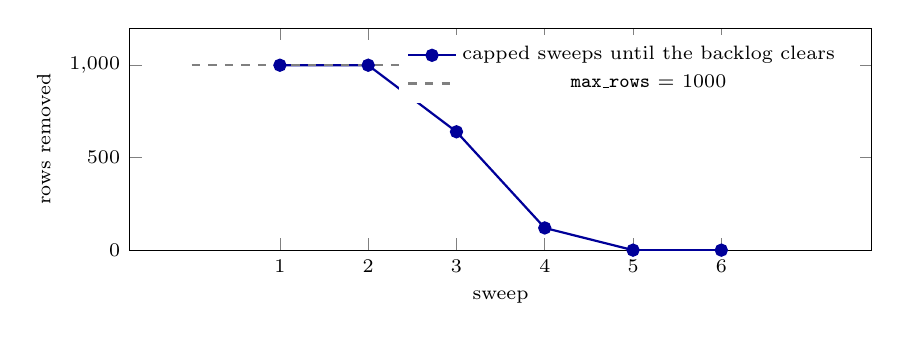
\begin{tikzpicture}
	\begin{axis}[
		width=11cm, height=4.4cm,
		xlabel={sweep}, ylabel={rows removed},
		ymin=0, ymax=1200,
		xtick={1,2,3,4,5,6},
		xlabel style={font=\scriptsize},
		ylabel style={font=\scriptsize},
		tick label style={font=\scriptsize},
		legend style={font=\scriptsize, draw=none},
		legend pos=north east,
	]
	\addplot[thick, mark=*, blue!60!black] coordinates {
		(1,1000) (2,1000) (3,640) (4,120) (5,0) (6,0)};
	\addlegendentry{capped sweeps until the backlog clears}
	\addplot[thick, dashed, gray, domain=0:7] {1000};
	\addlegendentry{\texttt{max\_rows} = 1000}
	\end{axis}
\end{tikzpicture}}
\captionof{figure}{The shape an operator should expect, illustrated, is several capped sweeps and
then quiet, while a store that reports 1\,000 on every sweep is receiving rows faster than the
policy expires them.}
\end{center}

\section{The queue store is a second store, with one writer}

The work queue is not a table in the run store. It is its own redb file with two tables ---
\texttt{queue\_item} keyed by item id and \texttt{queue\_event} keyed by \texttt{(id, seq)}
--- and a 4 MiB cache, in \texttt{crates/pii-store/src/queue.rs}. Keeping it separate means a
queue claim never competes for the write lock with a run's journal, and a store rebuilt for
one purpose does not have to be rebuilt for the other.

The single-writer rule shows up here in the protocol rather than in the process. The daemon is
the only writer; the CLI does not open the file. \texttt{pii queue add} sends a request over
the control socket, the engine's dispatch handles it, and the insertion and its
\texttt{queue.item.added} event are one transaction. A CLI that wrote the file directly would
be a second writer, and the daemon's in-memory view of the queue would be wrong until restart.

\begin{center}
\resizebox{\linewidth}{!}{%
\begin{tikzpicture}[node distance=8mm and 12mm]
	\node[b] (cli) {\texttt{pii queue add}};
	\node[b, right=of cli] (rpc) {socket request};
	\node[b, right=of rpc] (d) {daemon};
	\node[s, right=of d, yshift=8mm] (item) {queue\_item};
	\node[s, right=of d, yshift=-8mm] (ev) {queue\_event};
	\node[b, below=of d] (sched) {scheduler\\\scriptsize claim\_next};
	\node[b, right=of sched] (coder) {coder node};
	\node[b, below=of sched] (req) {requeue\_dead\_claims};

	\draw[f] (cli) -- (rpc);
	\draw[f] (rpc) -- (d);
	\draw[f] (d) -- (item);
	\draw[f] (d) -- (ev);
	\draw[f] (d) -- (sched);
	\draw[f] (sched) -- (coder);
	\draw[f] (req) -- node[p, right=2pt, midway]{dead claimant} (sched);
\end{tikzpicture}}
\captionof{figure}{One writer and one claim path, where the CLI reaches the store only through
the daemon and a claim is a status change plus its event in one transaction.}
\end{center}

\texttt{claim\_next} is the interesting method because it must be atomic against a second
caller. It opens one write transaction, reads every item, sorts by queue position, decides,
and --- only if the decision is a claim --- writes the item back as \texttt{Running} with its
attempt count incremented, its claimant recorded, and an \texttt{item.claimed} event appended,
all before the commit. A \texttt{Running} item short-circuits: the caller is told the queue is
already running something rather than being handed a second row.

\texttt{set\_status} follows the same shape: read the item, change its status, write it back,
journal \texttt{item.<status>} in the same transaction. That is what makes the queue's event
log sufficient to explain any row's state without reconstructing it from logs elsewhere.

\texttt{requeue\_dead\_claims} is the recovery path. It asks a caller-supplied predicate
whether the recorded claimant of a \texttt{Running} row is dead (an empty string for a row
with no recorded claim), returns those rows to \texttt{Pending}, and journals each as
\texttt{requeued\_after\_restart}. The returned count is what the daemon reports at boot. Two
properties matter: the predicate is supplied by the caller, so the store does not need to know
how to look up a process, and a row whose claimant is alive is left alone, so a second daemon
cannot steal work from a running one.

\begin{lstlisting}[language=bash]
pii queue add --id 376 --spec specs/376-retention-drops-what-the-policy-expires.md \
              --title "retention drops what the policy expires" \
              --criteria "cargo test -q -p pii-store --test retention_drops_what_the_policy_expires" \
              --touches crates/pii-store/src/retention.rs
pii queue ls
pii queue claim --by operator
\end{lstlisting}

\section{Bounded artefacts}

A store is one of several things a long-lived host fills. \texttt{pii disk} prints the others
in one table: the warm gate cache, the fresh-gate target, the coverage and tool target dirs,
the trash that parks work, and the gate exports outside the repository, each with bytes, age,
and \emph{the filesystem it sits on}. The filesystem column exists because a floor was once
measured on the wrong volume: two cleans freed 150 GB where nothing was short.

\begin{itemize}
	\item \texttt{\_tmp/gate-target} --- the warm build cache every gate step shares;
	\item \texttt{\_tmp/gate-target-fresh} --- the \texttt{--fresh} export's separate cache;
	\item \texttt{\_tmp/targets} --- per-step target dirs (clippy, doctest, tools);
	\item \texttt{\_tmp/\_trash} --- in-repo quarantined work;
	\item \texttt{/projects/\_tmp} --- \texttt{fresh-gate-<pid>} exports;
	\item \texttt{/projects/\_trash} --- quarantined working trees, one directory per park;
	\item \texttt{/tmp/\_trash-podman} --- container scratch that outlives a run;
	\item \texttt{/tmp/gate-cache} --- tool caches outside the repository.
\end{itemize}

Each row carries bytes, age and the owning filesystem, because the question an operator asks
is not ``how big is this'' but ``which volume is short''.

Each has an owner and a ceiling. The warm cache is capped at 40 GiB by
\texttt{FRESH\_GATE\_CACHE\_MAX\_GB}, and is trimmed before a build only when no cargo or
rustc is live --- a running build would lose its target under it. The trajectory directory is
bounded by bytes and file count (512 MiB and 50\,000 by default) and prunes the oldest
finished runs. The store's own page cache is 8 MiB, which is the subject of the next section.

\section{The two numbers that were wrong}

\paragraph{The page cache.} redb defaults to a 1 GiB cache. For a control-plane daemon holding
a store of a few megabytes that is not a tuning detail; under soak it appeared as a slow,
sublinear RSS climb with a flat thread count, a flat descriptor count, and a store file of a
few megabytes. The climb was in no code that owned a connection or a thread. Setting the cache
to 8 MiB left ample headroom under the 50 MB budget the RSS gate enforces.

\paragraph{The index nothing read.} \texttt{RESUME\_INDEX} was declared in \texttt{tables.rs},
opened three times in \texttt{lib.rs}, written by the scheduler's dispatch path, and counted
into the identity stats. The code's own comment at the write site said that nothing read it.
The cost was real --- an index write on every resume --- and the number invited an operator to
trust a structure with no reader. Spec 375 removed the table, every \texttt{open\_table}, the
write site, and the stat, while explicitly keeping \texttt{RUN\_JOURNAL} and
\texttt{RUN\_BY\_STATUS}, which are read. The guardrail in that spec is the useful part for a
reviewer: do not drop a table because it looks unused; drop it because you found the reader
that does not exist.

\section{Format version and identity}

A store records a format version in \texttt{meta}. Opening a store whose recorded version is
\emph{newer} than the binary understands is refused with both numbers in the message, so an
old binary never writes into a layout it does not know. A fresh or pre-versioning store is
stamped on open. The auxiliary stores --- approvals, heal, memory, channel, timer, queue ---
are stamped the same way through one shared function, so there is one rule and not six.

\texttt{Store::info} reports the path, the file size, the format version, the last write time,
and per-table entry counts. It counts six tables, not all of them: \texttt{graph\_body},
\texttt{run}, \texttt{run\_journal}, \texttt{run\_snapshot}, \texttt{session},
\texttt{session\_msg}. That is a deliberate short list --- the counts an operator needs to
answer ``is this store growing, and in which of the two big things'' --- and \texttt{pii store
stats} surfaces it. The health record carries the same numbers under \texttt{entries.<table>},
so a probe can compare two hosts without reading either store.

\begin{lstlisting}[language=bash]
pii store stats
pii store compact      # daemon stopped
pii store prune        # daemon stopped
\end{lstlisting}

\section{What a single run writes}

A worked example makes the accounting concrete. One run of a four-node graph, with two node
calls, writes the following (an illustrative count, not a captured run):

\begin{itemize}
	\item one row in \texttt{run} (rewritten on every append, so the header is the hot row);
	\item one \texttt{run\_journal} row per event: started, node started, node finished, node
	started, node finished, finished --- six rows for four nodes, because the run itself emits
	two;
	\item one \texttt{run\_by\_status} entry, rewritten as the status moves, and removed from
	the old status bucket each time;
	\item one \texttt{sys\_status\_run} row and one rewrite of the \texttt{sys\_status} totals;
	\item zero \texttt{graph\_body} rows on the second and later runs of the same graph,
	because the body is already stored under its hash.
\end{itemize}

The header being hot is why the append path rewrites it once per call rather than once per
event: batching events into one append is what keeps a chatty node from paying a header write
per event.

\section{Failure modes worth recognising}

\begin{enumerate}
	\item \textbf{A second writer.} Two processes on one store interleave writes or refuse; the
	symptom is a lock error naming the file, usually from a test that inherited the operator's
	\texttt{PII\_STATE\_DIR}. The fix is that every test daemon owns its own state directory.
	\item \textbf{A counter that lags.} A health number that changes only after a restart means
	the observer is installed after the first writes, or is not installed at all. The rebuild
	walk is how to tell lag from corruption.
	\item \textbf{A sweep that deletes what it cannot date.} Symptom: a store that loses its
	oldest and most interesting runs first, and a fixture that fails only with seeded pre-clock
	rows.
	\item \textbf{A sweep that blocks.} Symptom: every append stalls for the duration of one
	sweep. The cap is the fix, and a sweep that reports exactly 1\,000 is the evidence that it
	is working.
	\item \textbf{A table with no reader.} Symptom: a statistic nobody can act on, and a write
	cost on a hot path. The test is to delete the table and see whether any test fails for the
	right reason.
	\item \textbf{A cache that grows toward its default.} Symptom: RSS climbing with flat
	threads and flat descriptors, no leak in any owner. Check the embedded database's cache
	before rewriting the connection pool.
\end{enumerate}

Each of these was observed here, and each is now pinned by a test that fails if the fix is
reverted: the transaction count for id blocks, the transaction count for a duplicate graph
body, the undateable-row fixture, the live-run fixture, and the identity report.

\chapter{The daemon}

\label{ch:daemon}

This chapter answers what the daemon is, what it refuses to start without, and where the real
security boundary sits. The short answer: one process per state directory, one writer per
store, a socket for everything else, and a filesystem confinement applied before the first
byte is served. The interesting part is not the wiring diagram; it is the order of the checks,
because each check exists to make a specific failure impossible rather than unlikely.

\section{The production shape}

Four binaries ship: \texttt{pii}, \texttt{pii-mcp}, \texttt{pii-web} and \texttt{pii-evolve}.
The daemon is not a fifth. \texttt{pii} embeds it in-process, so \texttt{pii daemon} runs the
control plane in the foreground and \texttt{pii -p}, \texttt{pii tui} and the command surface
either talk to a running daemon over the control socket or start an engine of their own. There
is one engine implementation and no client-side copy of the rules.

\begin{center}
\resizebox{\linewidth}{!}{%
\begin{tikzpicture}[node distance=8mm and 12mm]
	\node[b] (cli) {\texttt{pii-cli}};
	\node[b, right=of cli, xshift=6mm] (daemon) {daemon\\\scriptsize one writer};
	\node[s, right=of daemon, yshift=12mm] (store) {store.redb};
	\node[s, right=of daemon, yshift=-12mm] (dur) {durable/\\\scriptsize channel $\cdot$ timer};
	\node[b, below=of daemon] (sandbox) {sandbox\\\scriptsize landlock profile};
	\node[b, right=of sandbox] (worker) {worker\\\scriptsize agent argv};
	\node[b, left=of sandbox] (caps) {capability set\\\scriptsize ceiling $\cap$ node caps};
	\node[b, above=of daemon] (log) {daemon log\\\scriptsize JSON lines};

	\draw[f] (cli) -- node[p, above=2pt, midway]{socket} (daemon);
	\draw[f] (daemon) -- (store);
	\draw[f] (daemon) -- (dur);
	\draw[f] (daemon) -- (sandbox);
	\draw[f] (caps) -- (sandbox);
	\draw[f] (sandbox) -- (worker);
	\draw[f] (daemon) -- (log);
\end{tikzpicture}}
\captionof{figure}{One binary, one writer, a socket, and two independent bounds between the
engine and any agent: the process-wide sandbox and the per-node capability set.}
\end{center}

The two bounds are worth separating at the start because they answer different questions. The
capability set answers ``may this node do this kind of thing'' --- read files, write files,
reach the network, spawn a process. The sandbox answers ``may this process, at all'' --- and
it is enforced by the kernel, after the engine has decided. A node without \texttt{fs\_write}
cannot write whatever the agent believes about itself, and an agent that talks its way past
its own instructions still cannot write outside the granted paths.

\section{Boot order}

The order is the chapter's real subject. Each step below can refuse, and each refusal names
the thing that failed before anything has been bound, spawned or written.

\begin{enumerate}
	\item \textbf{Flags and config.} \texttt{pii daemon} takes \texttt{--store},
	\texttt{--config}, \texttt{--workspace}, \texttt{--sandbox}, \texttt{--log-file}. An
	unknown key in the config file is a load error, not a silent default: a typo'd grant must
	not become no grant.
	\item \textbf{The sandbox.} Under \texttt{--sandbox workspace}, confinement is applied and
	verified before the store is opened. Failure exits \texttt{4}.
	\item \textbf{The measurement switches.} \texttt{--observer} and \texttt{--audit} accept
	\texttt{on} or \texttt{off}; a typo is an error, never ``on''.
	\item \textbf{The log and the starting mark.} \texttt{daemon.starting} is written before
	anything that can fail, carrying the pid and the store parent, so a start that never serves
	is visible in the record rather than only in the supervisor's journal.
	\item \textbf{The durable claim.} \texttt{pii\_store::durable::claim} probes
	\texttt{channel.redb} and \texttt{timer.redb}; a store another process holds exits
	\texttt{3} with the store's path in the message.
	\item \textbf{The model.} No model configured exits \texttt{5}. The daemon will not start
	into a state where the first agent dispatch is the thing that discovers the omission.
	\item \textbf{The store and the engine.} One retention sweep runs here; a failure is
	reported as \texttt{store.retention.failed} and is not a refusal.
	\item \textbf{Channels, MQTT, cron, workers.} Each entry is validated; a cron entry whose
	graph does not start at a \texttt{timer} node is refused, because it would re-run as fast
	as it finishes.
	\item \textbf{The socket.} Bound last, after everything the daemon needs is known good.
\end{enumerate}

\begin{center}
\resizebox{\linewidth}{!}{%
\begin{tikzpicture}[node distance=8mm and 12mm]
	\node[b] (flags) {flags\\\scriptsize exit 2};
	\node[b, right=of flags] (sb) {sandbox\\\scriptsize exit 4};
	\node[b, right=of sb] (mark) {daemon.starting};
	\node[b, right=of mark] (claim) {durable claim\\\scriptsize exit 3};
	\node[b, below=of claim] (model) {model\\\scriptsize exit 5};
	\node[b, left=of model] (store) {store + engine\\\scriptsize sweep};
	\node[b, left=of store] (entries) {channels $\cdot$ cron\\\scriptsize validated};
	\node[b, left=of entries] (sock) {socket\\\scriptsize bound last};

	\draw[f] (flags) -- (sb);
	\draw[f] (sb) -- (mark);
	\draw[f] (mark) -- (claim);
	\draw[f] (claim) -- (model);
	\draw[f] (model) -- (store);
	\draw[f] (store) -- (entries);
	\draw[f] (entries) -- (sock);
	\draw[bk] (sb.north) -- ++(0,6mm) node[p, above=2pt, midway]{refuse};
\end{tikzpicture}}
\captionof{figure}{Every refusal happens before the socket exists, so a start that fails fails
where a person is watching a terminal rather than on the first request from a client.}
\end{center}

\begin{longtable}{@{}p{0.10\textwidth}p{0.34\textwidth}p{0.46\textwidth}@{}}
\toprule
\textbf{Exit} & \textbf{Condition} & \textbf{Message shape} \\
\midrule
\endhead
2 & bad flag or config & \texttt{config: <toml error>} or the usage line \\
3 & a durable store is held & \texttt{store <path> is locked: another daemon holds it} \\
4 & sandbox not enforceable & \texttt{sandbox: enforcement could not be verified} \\
5 & no model configured & \texttt{no model configured (set PII\_MODEL, or [core].model ...)} \\
\bottomrule
\end{longtable}

\begin{lstlisting}[language=bash]
pii daemon --store /var/lib/pii/store.redb \
           --workspace /projects/pi-improved \
           --sandbox workspace \
           --config ~/.pii/pii.toml \
           --log-file /var/log/pii/daemon.jsonl
\end{lstlisting}

The default store path is documented in the flags' own help as \texttt{<runtime
dir>/store.redb}, and the default workspace is the working directory. The defaults are the
thing to check when a daemon ``sees the wrong data'': the store path decides which history a
client is reading, and the workspace decides which files a sandboxed agent may write.

\section{One writer, enforced three times}

The store admits one process. That sentence is true at three levels, and each level catches a
different mistake.

\paragraph{The database file.} redb takes an exclusive lock on the file. A second process that
opens it either blocks or fails; either way two processes never interleave writes. The
single-writer rule in \texttt{pii-store} is about transactions inside one process; the file
lock is about processes.

\paragraph{The durable pair, claimed first.} The channel cursor and the timer wheel are
separate small databases under the state directory. Before binding anything, the daemon probes
both with a non-blocking lock, one attempt per store, no retry, no create. A store that is
free is left exactly as it was found; a store that is held is named. The probe deliberately
keeps no lock --- the owner opens the store immediately after --- so the claim is a check, not
a reservation.

\paragraph{The state directory.} \texttt{PII\_STATE\_DIR} is resolved before \texttt{HOME}, so
a second instance --- a test, a soak, an operator's second daemon --- opens its own store, its
own durable pair and its own audit log. Without that resolution order, a test started beside a
running daemon opens the operator's \texttt{channel.redb}, finds it held, and hangs before
binding its socket. The symptom is a test that never starts and a daemon log with nothing in
it.

\begin{center}
\resizebox{\linewidth}{!}{%
\begin{tikzpicture}[node distance=8mm and 12mm]
	\node[b] (a) {daemon A\\\scriptsize state dir S};
	\node[b, right=of a, yshift=10mm] (sa) {S/store.redb};
	\node[b, right=of a, yshift=-10mm] (da) {S/durable/};
	\node[b, below=of a] (b) {daemon B\\\scriptsize state dir S};
	\node[b, right=of b, yshift=-10mm] (ref) {refusal\\\scriptsize exit 3};
	\node[b, right=of b, yshift=10mm] (sb) {S/store.redb};

	\draw[f] (a) -- (sa);
	\draw[f] (a) -- (da);
	\draw[bk] (b) -- node[p, below=2pt, midway]{claim} (ref);
	\draw[sf, dashed] (sb) -- (sa);
	\node[p, right=of sa, xshift=2mm, font=\scriptsize\itshape, align=left]
{held by A};
\end{tikzpicture}}
\captionof{figure}{The second daemon is refused by name rather than queued behind a lock,
because waiting produced a hang with no message that reads as a broken binary.}
\end{center}

The rule has a cost the operator must know: two daemons cannot share a state directory, so two
concurrent soaks or two test suites need two directories. The failure when they do not is loud
now, which is the point; before it was loud, it was a flaky test attributed to the code under
test.

\section{Two directories that mean different things}

The runtime directory holds things that are allowed to vanish on reboot:
\texttt{control.sock}, the graphs a daemon loads, \texttt{crashes/}. On this host it is a
per-user directory under \texttt{/run/user}. The state directory holds things that must
survive: the run store, the durable pair, the audit log.

Keeping them apart is a decision with a visible consequence. A store under the runtime
directory would be emptied by a reboot, and a reboot would therefore silently delete every run
history and every pending timer. The durable directory is resolved as
\texttt{[core].durable\_dir} when set, else \texttt{<state\_dir>/durable}, and never defaults
to the runtime directory. The comment in \texttt{daemon/mod.rs} says why in one clause: the
runtime dir is a tmpfs.

\section{The sandbox is the real bound}

\texttt{crates/pii-tools/src/sandbox.rs} implements two profiles and one rule about them.

\begin{longtable}{@{}p{0.14\textwidth}p{0.78\textwidth}@{}}
\toprule
\textbf{Profile} & \textbf{What is in force} \\
\midrule
\endhead
\texttt{workspace} & WRITES confined to the workspace, the store directory, the runtime directory,
\texttt{\$TMPDIR}, the container runtime state dirs and \texttt{/dev/shm}, plus the device
files \texttt{/dev/null}, \texttt{/dev/zero}, \texttt{/dev/urandom}, \texttt{/dev/tty}. READS
are not confined: read-only access to \texttt{/} is granted, so \texttt{/etc}, \texttt{HOME}
and every other
readable path stay readable. \\
\texttt{off} & no filesystem confinement in force; the explicit opt-out. Reported loudly at start,
in the log, in the audit trail and by \texttt{pii health}. \\
\bottomrule
\end{longtable}

The asymmetry --- writes confined, reads not --- is stated in the same words in four places:
the profile's grant text, the startup event, \texttt{pii health}, and the deploy runbook. One
text, so a reader cannot get a more generous impression from one surface than another. The
test suite pins the wording, which is unusual and deliberate: a permission model that is
described differently in two places is two permission models.

Applying the profile is \texttt{apply\_workspace}, and it is fail-closed in a way worth
reading line by line.

\begin{enumerate}
	\item The ruleset handles every filesystem access the ABI knows, and is created before any
	rule is added. A failure here is an error, not a partial ruleset.
	\item Every read-only path (\texttt{/} and \texttt{/dev}) is added as read access. A
	missing path is skipped rather than fatal, because a container may not have it.
	\item Every writable path is added with full directory rights --- except device nodes,
	which get file-content rights only. Granting directory rights on a device file makes the
	kernel downgrade the whole ruleset to partially enforced, which would silently weaken
	everything else.
	\item The ruleset is applied to the process. If the resulting status is not fully enforced,
	or \texttt{no\_new\_privs} is not set, the function returns an error. The caller exits
	\texttt{4}.
	\item An \emph{out-of-grant} probe writes a file in a directory that must not be writable.
	If the write succeeds, confinement is not real and the function fails.
	\item An \emph{in-grant} probe writes a file in a directory that must be writable. If that
	write fails, the grant is inert --- every rule was skipped or downgraded --- and the
	function fails.
\end{enumerate}

\begin{center}
\resizebox{\linewidth}{!}{%
\begin{tikzpicture}[node distance=8mm and 12mm]
	\node[b] (rules) {ruleset\\\scriptsize ro: / and /dev};
	\node[b, right=of rules] (rw) {rw: listed dirs\\\scriptsize files get content rights};
	\node[b, below=of rw] (restrict) {\texttt{restrict\_self}};
	\node[v, below=of restrict] (status) {enforced?};
	\node[b, left=of status] (exit) {exit 4};
	\node[b, below=of status] (out) {out-grant probe\\\scriptsize must fail};
	\node[b, below=of out] (in) {in-grant probe\\\scriptsize must succeed};
	\node[b, left=of in] (serve) {serve};

	\draw[f] (rules) -- (rw);
	\draw[f] (rw) -- (restrict);
	\draw[f] (restrict) -- (status);
	\draw[f] (status) -- node[p, above=2pt, midway]{yes} (out);
	\draw[bk] (status) -- node[p, above=2pt, midway]{no} (exit);
	\draw[f] (out) -- (in);
	\draw[f] (in) -- node[p, above=2pt, midway]{ok} (serve);
	\draw[bk] (in.south) |- node[p, below=2pt, midway]{inert} (exit.south);
\end{tikzpicture}}
\captionof{figure}{Six checks, two of them probes in opposite directions, because without the
in-grant probe a ruleset whose every rule was skipped would pass the out-grant test while
granting nothing, and every later refusal becomes a coincidence.}
\end{center}

The two probes are the part that survives review. A single out-grant probe proves that
something is denied; it cannot distinguish ``confined correctly'' from ``confined to
nothing''. The in-grant probe is the control that makes the first probe meaningful, and it is
the reason a report of a green sandbox on a new host can be trusted.

\paragraph{Two grants that are not obvious.} Podman keeps its graph root under
\texttt{HOME/.local/share/containers} and its runroot and locks under
\texttt{XDG\_RUNTIME\_DIR/containers} and \texttt{XDG\_RUNTIME\_DIR/libpod}. A sandboxed
daemon without those could not inspect a present image: the measured symptom was
\texttt{EACCES} on \texttt{bolt\_state.db} and \texttt{alive.lck}. The fourth entry is
\texttt{/dev/shm}, because podman's rootless lock file lives there and the profile grants
\texttt{/dev} read-only. The podman \emph{socket} is deliberately not a grant: a process
reaches it by \texttt{connect()}, which landlock does not mediate, so adding it would change
the grant text without changing what is allowed. A test asserts the text does not mention it,
which keeps the documentation and the mechanism from drifting apart.

\paragraph{The forced-failure switch.} \texttt{PII\_SANDBOX\_FORCE\_UNSUPPORTED=1} makes
\texttt{apply\_workspace} return the unverifiable error immediately. It exists so the exit-4
path can be exercised on a host where landlock \emph{does} work --- a refusal path that is
never run is a refusal path that does not work.

\section{The capability ceiling}

The sandbox is process-wide and coarse. The capability set is per-run and per-node, and it is
the bound an agent's own instructions cannot argue with.

A capability set is twelve bits plus five scopes. The bits are stable forever, because a
worker or a plugin references them without depending on the engine:

\begin{longtable}{@{}p{0.16\textwidth}p{0.06\textwidth}p{0.66\textwidth}@{}}
\toprule
\textbf{Kind} & \textbf{Bit} & \textbf{What it permits} \\
\midrule
\endhead
\texttt{fs\_read} & 1 & read files within an allow path scope \\
\texttt{fs\_write} & 2 & write files within an allow path scope \\
\texttt{net} & 4 & reach the network \\
\texttt{proc} & 8 & spawn or talk to processes \\
\texttt{hw} & 16 & touch hardware \\
\texttt{secrets} & 32 & access secrets \\
\texttt{memory\_write} & 64 & write into the agent's memory \\
\texttt{spawn} & 128 & spawn subprocesses \\
\texttt{memory\_read} & 256 & read from the agent's memory \\
\texttt{post} & 512 & post into a configured channel \\
\texttt{mqtt\_read} & 1024 & list and subscribe to a house's devices \\
\texttt{mqtt\_write} & 2048 & command a device through its allowlist \\
\bottomrule
\end{longtable}

The only operation on two sets is intersection. There is deliberately no union: a capability
set can be narrowed at every hop and widened at none. \texttt{CapSet::intersect} ANDs the bits
and intersects every scope; \texttt{narrow\_kinds} lowers the bits while keeping the inherited
path and host scopes, which is what a node that declares fewer capabilities than its run gets.

On top of the per-run set sits a ceiling from configuration: \texttt{[grant\_ceiling]} names
the capability kinds no graph or node may request beyond. An empty list means no ceiling; a
name the engine does not know is an invalid-config error rather than a silently ignored entry.
The check runs where the node is built, so a graph asking for more than the ceiling is refused
before it runs, and the refusal names the capability.

Path scopes are deny-wins. \texttt{PathScope::permits} checks the deny list first, so a path
inside an allow prefix but inside a deny prefix is refused. The heal path uses that to keep a
patch away from \texttt{specs}, \texttt{xtask}, \texttt{quality-gate.sh}, \texttt{graphs},
\texttt{clippy.toml}, \texttt{rust-toolchain.toml} and \texttt{.github}: a heal worktree is a
full checkout, and without the deny list a patch could delete the assertions that prove it
worked.

\begin{lstlisting}[language=bash]
[core]
model = "llamacpp-server:granite-4.2-3b"

# the ceiling: no graph or node may request beyond these kinds
grant_ceiling = ["fs_read", "fs_write", "proc", "spawn", "net"]

[net]
grants = ["10.10.10.217:8082"]
allow_private = true

[[model_tier]]
name = "small"
model = "llamacpp-server:granite-4.2-3b"
tools = ["read_file", "grep"]
max_tokens = 2048
\end{lstlisting}

\paragraph{Why the two bounds are both needed.} A capability set with no sandbox is advice to
a process that has already been spawned by an engine with the operator's rights. A sandbox
with no capability set confines a process but gives every node the same power inside the
fence. The pairing is what makes ``this node may write, that node may not, and neither may
write outside the workspace'' expressible.

\section{The socket, and why clients are thin}

Every client reaches the daemon through one unix socket, \texttt{control.sock}, under the
runtime directory. The socket is the boundary that keeps a second copy of the rules from
existing: \texttt{pii run ls}, \texttt{pii health}, \texttt{pii queue add} and \texttt{pii
skill show} all become a request with a method and a payload, and the engine answers. A client
cannot be more permissive than the daemon, because it has no engine of its own to be
permissive with.

The socket's location is computed once, from the runtime directory, and \texttt{pii-uds} owns
that computation --- one default socket, so a CLI started from a plain shell with no
environment finds the daemon that an operator started from a session with one. Before that,
\texttt{pii health} answered for a daemon that did not exist or failed to find one that did,
and the difference was an unset variable nobody could see.

This is also why a long-running command does not hold a store lock. The client sends a request
and waits; the work happens in the daemon, in the daemon's process, under the daemon's sandbox
and capability ceiling. The \texttt{--store} flag on a one-shot command exists for the case
where no daemon is running, and then the process really does open the file, which is why a
second one-shot beside a running daemon can collide where a socket request would not.

\section{What the daemon runs}

Beyond runs, the daemon owns a small set of long-lived things, each with its own failure mode:

\begin{itemize}
	\item \textbf{Channels} --- one runtime per configured channel, with a poll interval, a
	poll backoff and a graph to start per inbound message. The default poll interval is 1\,500
	ms because Discord answers a message read at roughly five requests per five seconds per
	route; at 500 ms the daemon collected 173 \texttt{channel.poll.failed 429} events in a few
	hours and never read a message.
	\item \textbf{MQTT connections} --- one broker connection each, subscribing to topic
	filters and starting a graph per message, with a bounded inbound queue that drops and
	counts beyond its cap. A name used by both a channel and an MQTT connection is a config
	error, not a last-writer-wins.
	\item \textbf{Cron entries} --- display-only schedules; the actual firing comes from the
	graph's entry \texttt{timer} node. The entry kind is checked at start, because a non-timer
	entry would re-run the instant it finishes.
	\item \textbf{Workers} --- declared in config as a program, its argv, extra environment and
	an in-flight cap, so a bounded number of external processes exist at once.
	\item \textbf{Timers} --- the durable wheel, rearmed from the store at boot.
	\item \textbf{Claim recovery} --- \texttt{requeue\_dead\_claims} at boot returns rows whose
	claimant is gone to \texttt{Pending}, so a killed daemon does not leave work claimed
	forever.
\end{itemize}

\section{Refusals that name the thing}

A refusal is only useful if it names what failed and where. The daemon's refusals follow one
shape: the object, the reason, and the identifier.

\begin{lstlisting}[language=bash]
store /root/.local/state/pii/durable/channel.redb is locked: another daemon holds it
cron 'nightly': graph 'night' must start at a timer node (entry is gate); it would re-run
  as fast as it finishes
config: [core].ollama_host is retired (spec 129) - set `[llama] host` for the
  llama.cpp server instead
config: duplicate [[model_tier]] name 'small'
sandbox: enforcement could not be verified
\end{lstlisting}

Two of those deserve comment. The retired \texttt{ollama\_host} key is refused \emph{by name}
rather than as an unknown field, because the generic message would send an operator looking
for a typo. And the duplicate tier name is refused at parse time, so a node asking for the
tier gets one provider rather than whichever entry happened to win.

\section{What an operator should check first}

When a daemon is suspected rather than proven wrong, four checks answer most questions without
reading code:

\begin{enumerate}
	\item \texttt{pii health --json}: the state of each subsystem, the store's path and
	per-table counts, and the mounts the process actually has.
	\item The log's first line: \texttt{daemon.starting} carries the pid and the store parent,
	so the process and the directory it opened are in the record.
	\item The sandbox line in \texttt{health}: \texttt{sandbox=workspace (landlock)} with the
	grants spelled out, or the loud \texttt{off} text.
	\item The store's parent directory, compared with \texttt{PII\_STATE\_DIR} and
	\texttt{HOME}: a daemon reading the wrong store looks exactly like a daemon with amnesia.
\end{enumerate}

\section{Failure modes worth recognising}

\begin{enumerate}
	\item \textbf{A test daemon that hangs on start.} Symptom: no socket, no log line after
	\texttt{daemon.starting}, a test that times out. Cause: it inherited the operator's
	\texttt{PII\_STATE\_DIR} and is waiting on a held \texttt{channel.redb}. Fix: give the test
	its own state directory.
	\item \textbf{A gate that fails on a channel lock.} Symptom: \texttt{channel.redb is
	locked: another daemon holds it} inside a gate run. Cause: the gate inherited a state dir
	from the shell that started it. The gate now removes \texttt{PII\_STATE\_DIR} and
	\texttt{PII\_RUNTIME\_DIR} from the child environment.
	\item \textbf{A sandbox that refuses every start.} Symptom: exit \texttt{4} on a host where
	landlock should work. Read the two probe outcomes: an out-grant write that succeeded means
	the ruleset did not apply; an in-grant write that failed means the grant list is wrong,
	usually a missing directory the process cannot create.
	\item \textbf{A podman run that cannot see its own image.} Symptom: \texttt{EACCES} on
	\texttt{bolt\_state.db}. Cause: the container state dirs are not in the grant list.
	\item \textbf{A node that ``has no write tool''.} Symptom: the agent stops and reports that
	no write or execute tool is available. Cause: the node declared too few capabilities --- a
	coder without \texttt{fs\_write} cannot implement anything. The fix is in the graph, not in
	the sandbox.
	\item \textbf{A cron entry that spins.} Symptom: a graph that starts again immediately
	after it finishes. Cause: the entry node is not a \texttt{timer}. The daemon refuses that
	at start now.
\end{enumerate}


\backmatter
\chapter{The habit that produced this manual}
Every mechanism described here was first understood by running it and then disbelieving its
explanation. The recurring failure in this codebase is not a missing feature; it is a
\emph{guard that fires on the case it exists to permit}, while reporting a reason that is
not the real one. Four instances appear in these chapters: a park that wedged the queue, a
dirty tree that refused its own work, a resolver nothing called, and a disk check that was
an unset variable.

The defence is the same each time: make the check consume what the live path actually
produces, and keep a control that must still take the normal path.

\end{document}
